
\chapter{Resultados del método East - West}

En este capítulo se presentan los resultados obtenidos mediante el método East-West con los eventos de Todos los Disparos, para  distintos rangos de energía. Estos resultados se comparan con los valores obtenidos en \cite{Aab_2020} sobre los eventos  del Disparo Estándar. 
% \section{Tabla cantidad de eventos para distintos rangos de energía}

Los eventos son clasificados en los distintos rangos mediante la energía reportada por la Colaboración. El conjunto de eventos registrados mediante de Todos los Disparos abarca eventos medidos entre el 2014 y 2019, y para el Disparo Estándar se listan eventos medidos entre el 2004 y 2018. Las características de estos dos conjuntos de datos se especifican en la Tabla \ref{tab:datasets}

\begin{table}[H]
    \begin{small}
        \begin{center}
            \begin{tabular}{lc|l|l|l|}
\hline
\multicolumn{1}{|l|}{\multirow{4}{*}{\begin{tabular}[c]{@{}c@{}}Rango \\ Tiempo\end{tabular}}}    & Todos       & Inicio &\multicolumn{2}{l|}{1 de Enero, 2014 } \\ \cline{3-5} 
\multicolumn{1}{|l|}{}                                                                            & 6 años      & Fin    &\multicolumn{2}{l|}{1 de Enero, 2020} \\ \cline{2-5} 
\multicolumn{1}{|l|}{}                                                                            & Estándar    & Inicio &\multicolumn{2}{l|}{1 de Enero, 2004} \\ \cline{3-5}
\multicolumn{1}{|l|}{}                                                                            & 14.8 años   & Fin    &\multicolumn{2}{l|}{1 de Octubre, 2018} \\ \hline  \\

\hline                                                                          \multicolumn{2}{|c|}{Rango [EeV]}                                                    & \multicolumn{1}{c|}{0.25 - 0.5}  & \multicolumn{1}{c|}{ 0.5  - 1 } &\multicolumn{1}{c|}{ 1 - 2 } \\ \hline
\multicolumn{1}{|l|}{\multirow{2}{*}{Eventos}}                            & Todos    & $3\,967\,368$     & $3\,638\,226$   & $1\,081\,846$ \\ \cline{2-5} 
\multicolumn{1}{|l|}{}                                                    & Estándar & $770\,323$        & $2\,388\,468$   & $1\,243\,098$ \\ \hline
\multicolumn{1}{|l|}{\multirow{2}{*}{\begin{tabular}[c]{@{}c@{}}Energía \\ Media\end{tabular}}} & Todos    & $0.38$           & $0.69$         & $1.32$       \\ \cline{2-5} 
\multicolumn{1}{|l|}{}                                                                             & Estándar & $0.42$            & $0.71$          & $1.34$       \\ \hline
\end{tabular}
            \caption{Características de los conjuntos de datos para distintos rangos de energía }
            \label{tab:datasets}
        \end{center}
    \end{small}
\end{table}



\section{Resultados en distintos rangos de energía}
\subsection{Resultados en el rango 0.25 EeV - 0.5 EeV}

En la Tabla \ref{tab:primer_bin_data} se presentan los resultados para este rango de energía en las frecuencias solar y sidérea de Todos Los Disparos. Los mismos  se comparan con resultados con el Disparo Estándar que fueron reportados en \cite{Aab_2020}. En esta tabla se observa que las amplitudes $r$ en frecuencia sidérea no son compatibles dentro de los límites de confianza de cada uno. Los valores de $\sigma$ de Todos los Disparos es la mitad que el valor reportado para el Disparo Estándar,  esto se debe a que el primer conjunto de datos tiene registrados $\sim 5$  veces más eventos que el segundo.

\begin{table}[H]
    \begin{small}
        \begin{center}
            \begin{tabular}[c]{l|c|c||c|}
\cline{2-4}                                       & \multicolumn{2}{c||}{Todos los disparos}    & \multicolumn{1}{c|}{Disparo Estándar}   \\ \hline
\multicolumn{1}{|l|}{Frecuencia:                } & Solar	                & Sidérea	                & Sidérea \cite{Aab_2020}   \\ \hline
\multicolumn{1}{|l|}{Amplitud r [\%]:           } & $0.17^{+0.22}_{-0.07}$	& $0.12^{+0.24}_{-0.03}$ 	& $0.5^{+0.4}_{-0.2}$ \cite{codigo}      \\
\multicolumn{1}{|l|}{$r_{99}$ [\%]:             } & \multicolumn{2}{c||}{0.58}                          & 1.1\cite{codigo}                 \\
\multicolumn{1}{|l|}{$r^{UL}$ [\%]:             } & 0.67 	                & 0.64                      & 1.4\cite{codigo}                 \\ 
\multicolumn{1}{|l|}{$\sigma$[\%]:              } & \multicolumn{2}{c||}{0.19}                          & 0.38\cite{codigo}       \\\hline
\multicolumn{1}{|l|}{Amplitud $d_\perp$[\%]:    } & -	                    & $0.16^{+0.31}_{-0.04}$ 	& $0.6^{+0.5}_{-0.3}$       \\
\multicolumn{1}{|l|}{$d_{99}$ [\%]:             } & - 	                    & 0.73                      & 1.5  \cite{codigo}                \\
\multicolumn{1}{|l|}{$d_{\perp}^{UL}[\%]$       } & -                       & 0.80                      & 1.8                         \\
\multicolumn{1}{|l|}{$\sigma_{x,y}$[\%]:        } & -	                    & 0.24	                    & 0.48       \\\hline
\multicolumn{1}{|l|}{Probabilidad      :        } & 0.66                    & 0.81	                    & 0.45       \\
\multicolumn{1}{|l|}{Fase[$^o$]:                } & 221$\pm$93              & 280$\pm$124                & 225$\pm$64\\ \hline
\multicolumn{1}{|l|}{$\langle\cos\delta \rangle$} & \multicolumn{2}{c||}{0.79}        	                & 0.79 \cite{codigo}        \\        
\multicolumn{1}{|l|}{$\langle\sin\theta \rangle$} & \multicolumn{2}{c||}{0.46}        	                & 0.52 \cite{codigo}        \\ \hline       
            \end{tabular}
            
        \end{center}
    \end{small}
    \caption{Características para las frecuencias solar y sidérea con el método East-West en el primer armónico en rango de energía 0.25 EeV - 0.5 EeV.}
    \label{tab:primer_bin_data}
\end{table}


En la Fig. \ref{fig:primer} se comparan las  fases en frecuencia sidérea obtenida en este trabajo y la reportada en \cite{Aab_2020}, donde la línea punteada marca la dirección del centro galáctico.  En esta figura en la tabla anterior, se observa que la incertidumbre obtenida para la fase de Todos los Disparos es amplia, esto se debe a que la amplitud $r$ es pequeña comparada con el valor de $\sigma$. 


Realizando el barrido de frecuencias con la variable de la Ec.\ref{ra_arb}, se obtiene que en este rango de energía las amplitudes se  distribuyen en frecuencia como se muestra en la Fig.\ref{fig:primer_barrido}. La línea horizontal indica el valor de $r_{99}$ para cada frecuencia, además se observa que ninguna amplitud supera dicho umbral.

\begin{figure}[H]
    \begin{small}
        \begin{center}
            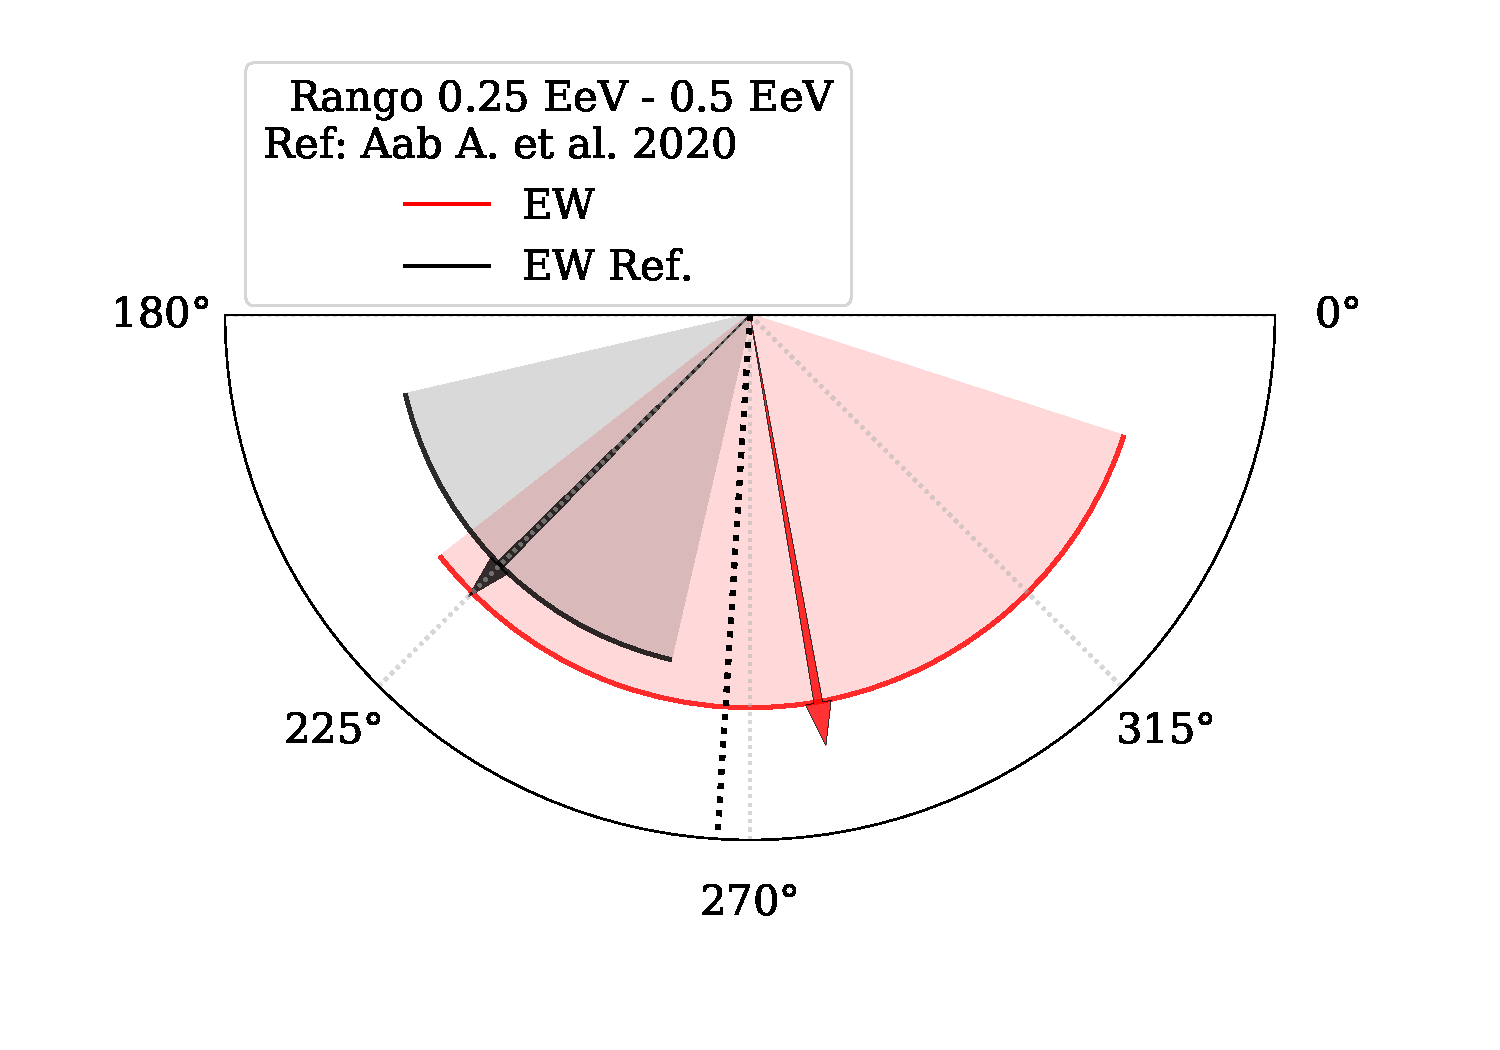
\includegraphics[width=0.75\textwidth]{phase_primer_bin_v2.pdf}
        \end{center}
        \caption{Valores de las fases obtenidos en este trabajo y en el trabajo \cite{Aab_2020} con sus respectivas incertidumbres para la frecuencia sidérea en el  rango 0.25 EeV - 0.5 EeV .}
        \label{fig:primer}
    \end{small}
\end{figure}

\begin{figure}[H]
    \begin{small}
        \begin{center}
            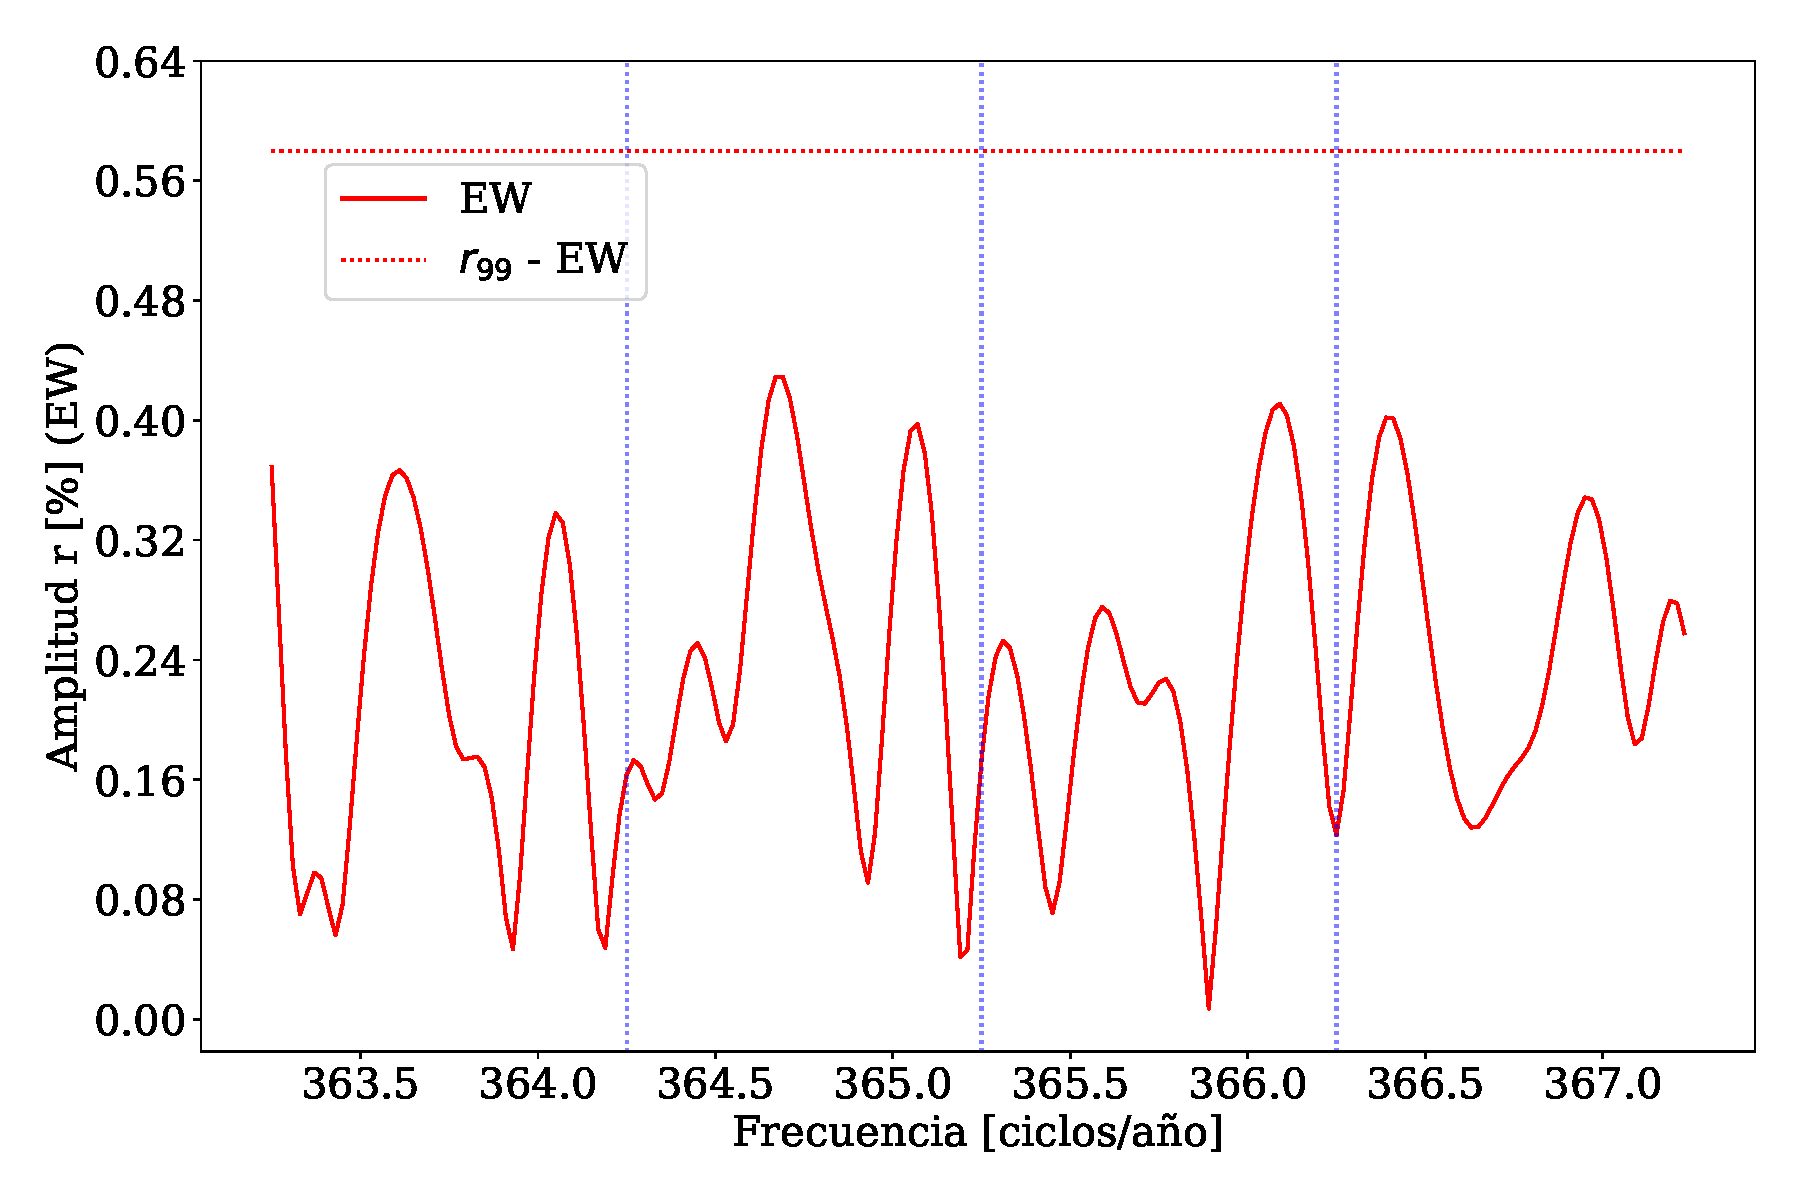
\includegraphics[width=0.75\textwidth]{plot_bin_1_barrido_v3_EW.pdf}
        \end{center}
        \caption{Barrido de frecuencias en el  rango 0.25 EeV - 0.50 EeV .}
        \label{fig:primer_barrido}
    \end{small}
\end{figure}

\subsection{Resultados en el rango 0.5 EeV - 1 EeV}
En la Tabla \ref{tab:primer_bin_data} se presentan los resultados para el rango 0.5 EeV - 1 EeV en las frecuencias solar y sidérea de Todos Los Disparos, además se comparan con los resultados reportados en \cite{Aab_2020}.


\begin{table}[H]
        \begin{small}
            \begin{center}
                \begin{tabular}[c]{l|c|c||c|}
\cline{2-4}                                       & \multicolumn{2}{c||}{Todos los disparos}    & \multicolumn{1}{c|}{Disparo Estándar}   \\ \hline
\multicolumn{1}{|l|}{Frecuencia:                } & Solar	                & Sidérea	                & Sidérea \cite{Aab_2020}   \\ \hline
\multicolumn{1}{|l|}{Amplitud r [\%]:           } & $0.43^{+0.21}_{-0.14}$	& $0.44^{+0.21}_{-0.14}$ 	& $0.38^{+0.20}_{-0.14}$ \cite{codigo}      \\
\multicolumn{1}{|l|}{$r_{99}$ [\%]:             } & \multicolumn{2}{c||}{0.56}                         & 0.64\cite{codigo}                 \\
\multicolumn{1}{|l|}{$r^{UL}$ [\%]:             } & 0.89 	                & 0.90                      & 0.90 \cite{codigo}                 \\ 
\multicolumn{1}{|l|}{$\sigma$[\%]:              } & \multicolumn{2}{c||}{0.18}                         & 0.21 \cite{codigo}      \\\hline
\multicolumn{1}{|l|}{Amplitud $d_\perp$[\%]:    } & -	                    & $0.56^{+0.27}_{-0.18}$ 	& $0.5^{+0.3}_{-0.2}$       \\
\multicolumn{1}{|l|}{$d_{99}$ [\%]:             } & - 	                    & 0.71                      & 0.8   \cite{codigo}                \\
\multicolumn{1}{|l|}{$d_{\perp}^{UL}[\%]$       } & -                       & 1.1                       & 1.1                         \\
\multicolumn{1}{|l|}{$\sigma_{x,y}$[\%]:        } & -	                    & 0.23	                    & 0.21       \\\hline
\multicolumn{1}{|l|}{Probabilidad      :        } & 0.065                   & 0.055	                    & 0.20       \\
\multicolumn{1}{|l|}{Fase[$^o$]:                } & 205$\pm$35              & 258$\pm$34                & 261$\pm$43\\ \hline
\multicolumn{1}{|l|}{$\langle\cos\delta \rangle$} & \multicolumn{2}{c||}{0.79}        	                & 0.79 \cite{codigo}        \\        
\multicolumn{1}{|l|}{$\langle\sin\theta \rangle$} & \multicolumn{2}{c||}{0.50}        	                & 0.54\cite{codigo}        \\ \hline       
                \end{tabular}
            \end{center}
        \end{small}
        \caption{Características para las frecuencias solar y sidérea con el método East-West en el primer armónico en rango de energía 0.5 EeV - 1 EeV}
        \label{tab:segundo_bin_data}
    \end{table}


    En la Fig. \ref{fig:segundo} se comparan las direcciones en las que apuntan la fase en frecuencia sidérea obtenida en este trabajo con la obtenida en \cite{Aab_2020}. En esta figura se observa que resultados similares entre sí en valor e incertidumbre, y apuntan a una dirección cercana al centro galáctico.

    El barrido de frecuencias con la variable de la Ec.\ref{ra_arb} para este rango de energía se observa en la Fig.\ref{fig:segundo_barrido}. La línea horizontal indica el valor de $r_{99}$ para cada frecuencia, además se observa que ninguna frecuencia supera dicho umbral. 
    
    \begin{figure}[H]
        \begin{small}
            \begin{center}
                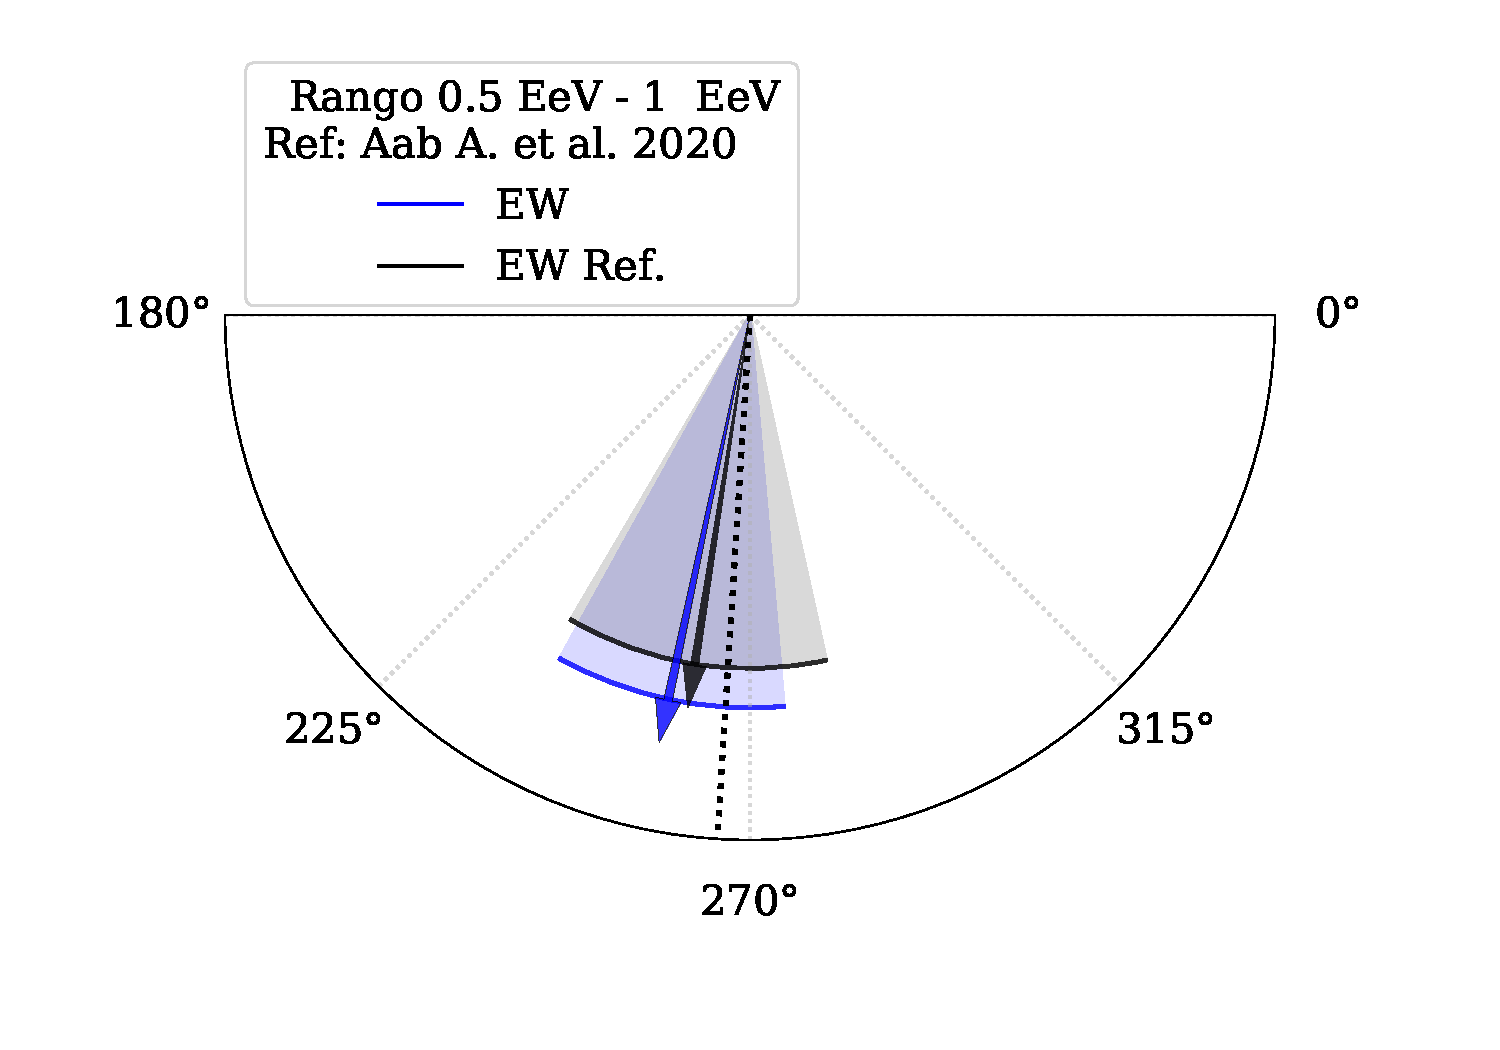
\includegraphics[width=0.75\textwidth]{phase_segundo_bin_v2.pdf}
            \end{center}
            \caption{Valores de las fases obtenidos en este trabajo y en el trabajo \cite{Aab_2020} con sus respectivas incertidumbres para la frecuencia sidérea en el rango 0.5 EeV - 1.0 EeV .}
            \label{fig:segundo}
        \end{small}
    \end{figure}


    \begin{figure}[H]
        \begin{small}
            \begin{center}
                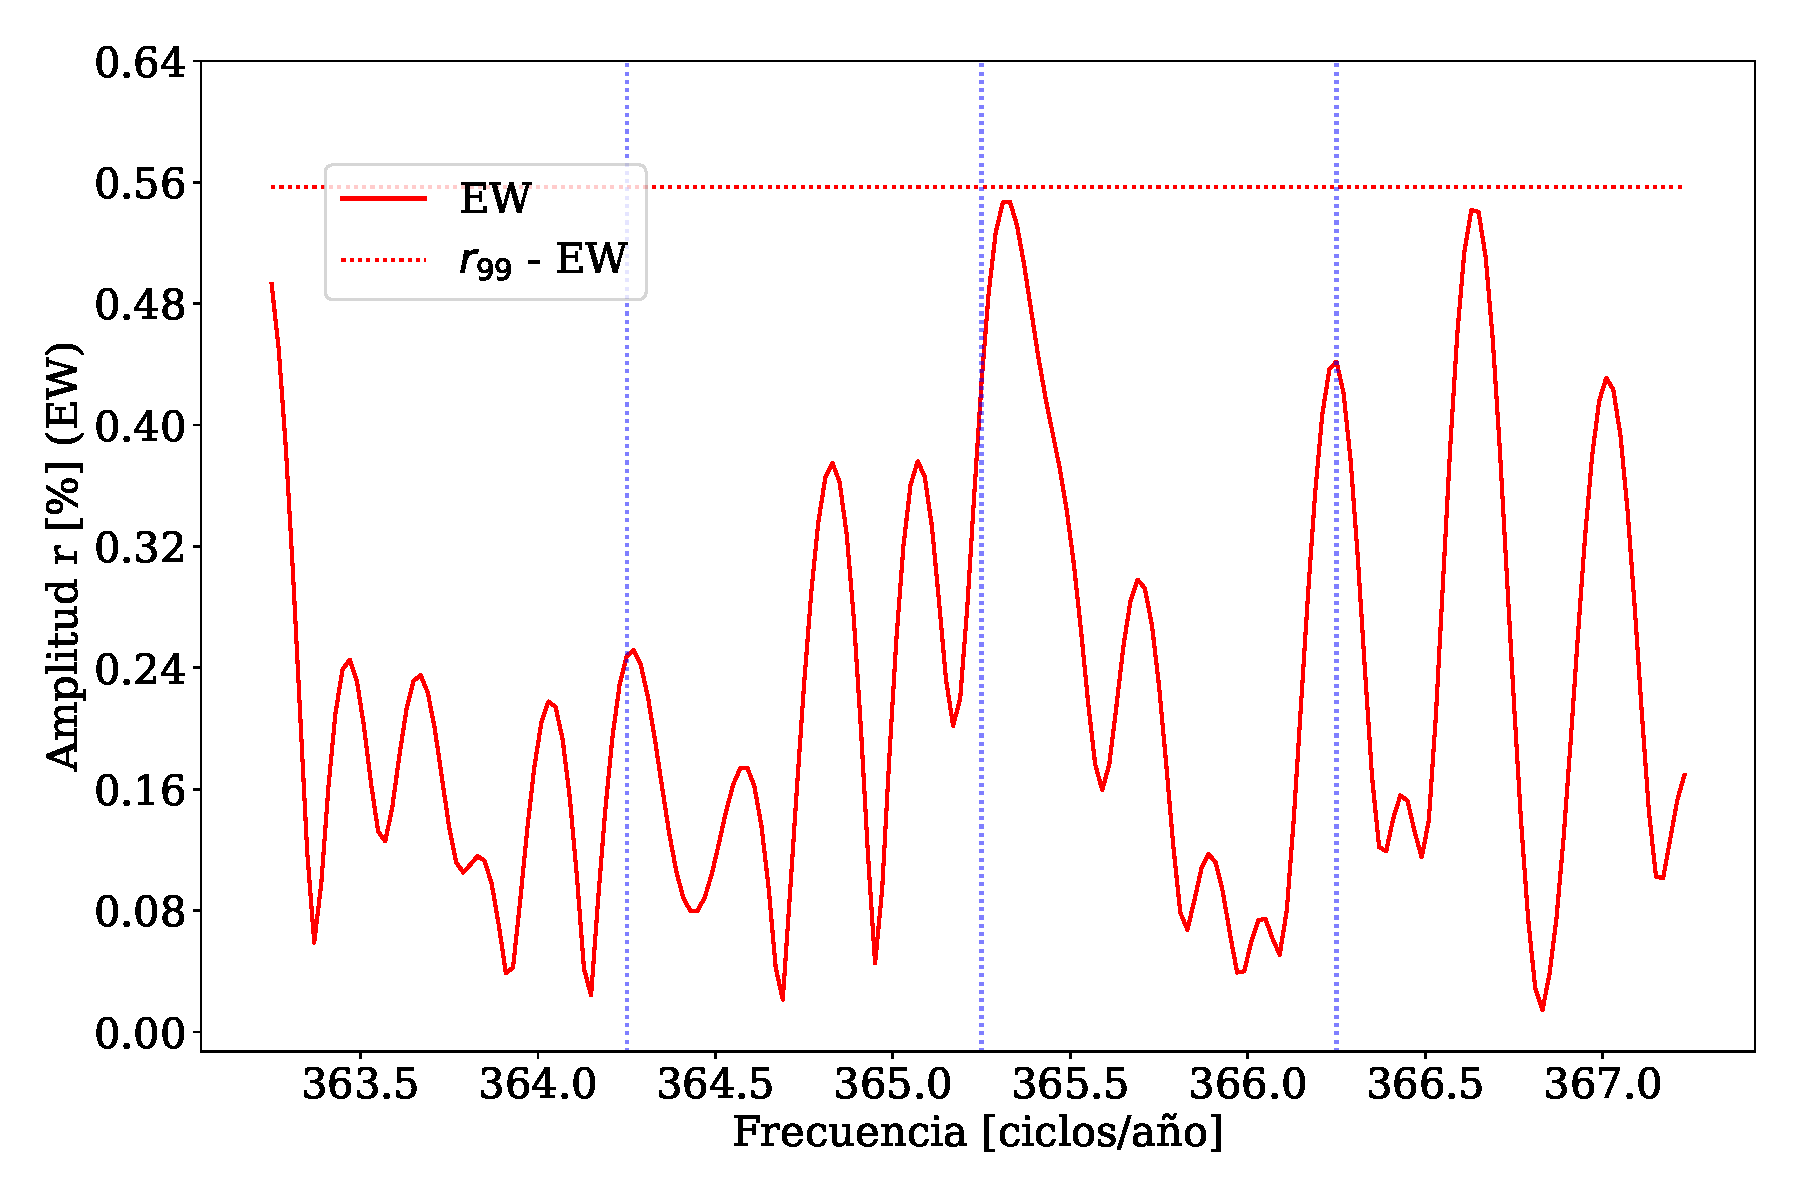
\includegraphics[width=0.75\textwidth]{plot_bin_2_barrido_v3_EW.pdf}
            \end{center}
            \caption{Barrido de frecuencias en el  rango 0.5 EeV - 1.0 EeV .}
            \label{fig:segundo_barrido}
        \end{small}
    \end{figure}    


\subsection{Resultados en el rango 1 EeV - 2 EeV}

 
En las Tablas \ref{tab:solar_3}  se comparan los resultados de este trabajo  para la frecuencia solar. Las amplitudes están por debajo de $r_{99}$ y con compatibles entre sí.

    \begin{table}[H]
        \begin{small}
            \begin{center}
                \begin{tabular}[c]{l|c|c|}
                    \cline{2-3}         & \multicolumn{2}{c|}{Todos los disparos} \\ \cline{2-3}
                                        & Rayleigh                      & East - West            \\\hline
\multicolumn{1}{|l|}{Frecuencia:}             &\multicolumn{2}{c|}{Solar}        \\
\multicolumn{1}{|l|}{Amplitud $r$[\%]:} & $0.24^{+0.16}_{-0.09}$        & $0.28^{+0.35}_{-0.11}$ \\
\multicolumn{1}{|l|}{$r_{99}$ [\%]:   } & 0.41                          & 0.91       \\
\multicolumn{1}{|l|}{$r_{UL}$ [\%]:   } & 0.58                          & 1.1       \\
\multicolumn{1}{|l|}{$\sigma$:        } & 0.14                          & 0.30          \\\hline
\multicolumn{1}{|l|}{Probabilidad:    } & 0.22                          & 0.65          \\
\multicolumn{1}{|l|}{Fase:            } & 260$\pm$48                    & 279$\pm$90    \\\hline
                \end{tabular}
            \end{center}
        \end{small}
        \caption{Características para la frecuencia solar con los métodos de Rayleigh  e East-West en el primer armónico.}
        \label{tab:solar_3}
    \end{table}
    
    En la Tabla \ref{tab:siderea_3} se comparan los resultados de este trabajo y los obtenidos en el trabajo \cite{Aab_2020} para la frecuencia sidérea. Para Todos los Disparos se comparan los métodos de Rayleigh y East-West, en el primer método se obtiene que la probabilidad que la amplitud obtenida se deba al ruido es de $6
    3\%$ mientras que en segundo método $26\%$. Esta diferencia entre probabilidades no puede deberse a la cantidad de eventos, porque es el mismo conjunto de datos. El método Rayleigh nos indica que en este rango de energía pueden existir efectos sistemáticos que no están siendo corregidos.


    \begin{table}[H]
        \begin{small}
            \begin{center}
                \begin{tabular}[c]{l|c|c||c|}
                    \cline{2-4}               &  \multicolumn{2}{c||}{Todos los Disparos}                  & Disparo Estándar      \\
                    \cline{2-4}               & Rayleigh                      & East - West                 & East - West\cite{Aab_2020}      \\\hline
\multicolumn{1}{|l|}{Frecuencia:             }& \multicolumn{2}{c||}{Sidérea}                               & Sidérea        \\ \hline
\multicolumn{1}{|l|}{Amplitud $r$ [\%]:      }& $0.32^{+0.16}_{-0.10}$ 	      & $0.5^{+0.3}_{-0.2}$         & $0.14^{+0.37}_{-0.02}$\cite{codigo}       \\
\multicolumn{1}{|l|}{$r_{99}$[\%]:           }& 0.41	                      & 0.91                        & 0.84\cite{codigo}        \\
\multicolumn{1}{|l|}{$r^{UL}[\%]$      }      & 0.66                          & 1.3                         & 0.89 \cite{codigo}        \\
\multicolumn{1}{|l|}{$\sigma$[\%]:     }      & 0.14                          & 0.30	                    & 0.28 \cite{codigo}          \\ \hline
\multicolumn{1}{|l|}{Amplitud $d_\perp$ [\%]:}& $0.41^{+0.20}_{-0.13}$        & $0.6^{+0.4}_{-0.3}$         & $0.18^{+0.47}_{-0.02}$       \\ 
\multicolumn{1}{|l|}{$d_{99}$[\%]:           }& 0.53	                      & 1.1                         & 1.1\cite{codigo}        \\
\multicolumn{1}{|l|}{$d_{\perp}^{UL}[\%]$    }& 0.84                          & 1.6                         & 1.1        \\
\multicolumn{1}{|l|}{$\sigma_{x,y}$[\%]:     }& 0.17                          & 0.38	                    & 0.35          \\ \hline
\multicolumn{1}{|l|}{Probabilidad:           }& 0.063	                      & 0.26                        & 0.87          \\
\multicolumn{1}{|l|}{Fase[$^o$]:             }& 357$\pm$35                    & 320$\pm$50                 & 291$\pm$100      \\\hline
\multicolumn{1}{|l|}{$\langle\cos\delta\rangle$} & \multicolumn{2}{c||}{0.78}                              & 0.78       \\        
\multicolumn{1}{|l|}{$\langle\sin\theta\rangle$} & \multicolumn{2}{c||}{0.55}                              & 0.57       \\ \hline       
\end{tabular}
            \end{center}
        \end{small}
        \caption{Características para la frecuencia sidérea con los métodos de Rayleigh  e East-West en el primer armónico.}
        \label{tab:siderea_3}
    \end{table}
   

    En el Fig.\ref{fig:tercer} se observan en un gráfico polar las fases del trabajo \cite{Aab_2020} y este trabajo para la frecuencia sidérea
    \begin{figure}[H]
        \begin{small}
            \begin{center}
                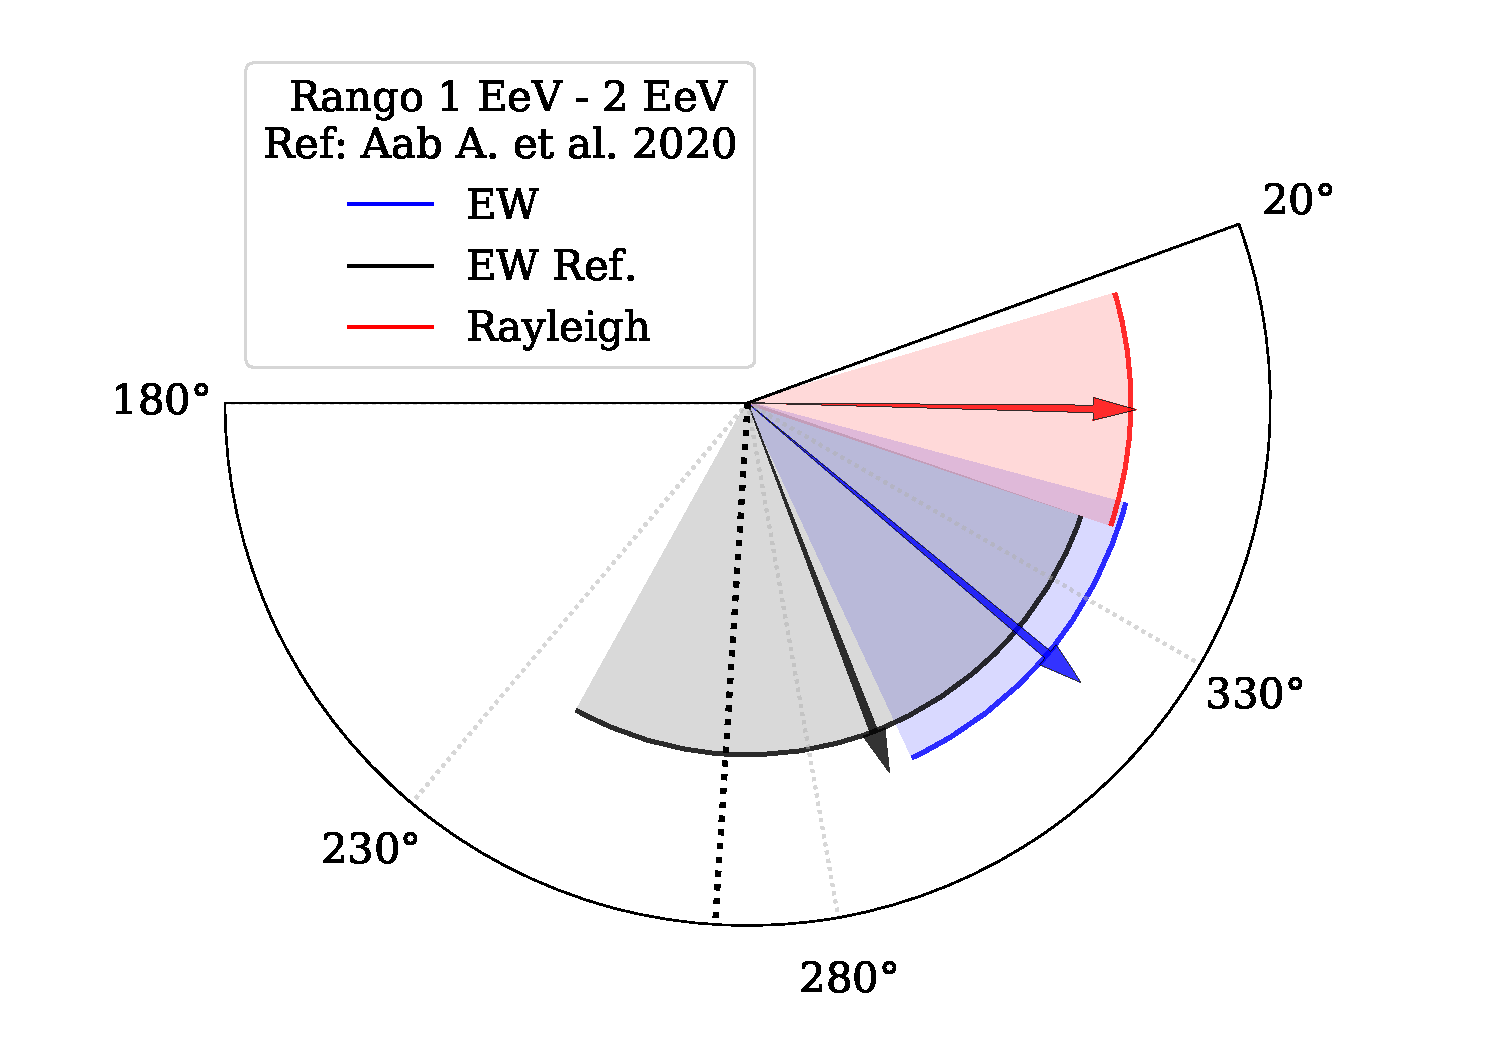
\includegraphics[width=0.75\textwidth]{phase_tercer_bin_v2.pdf}
            \end{center}
        \caption{Valores de las fases obtenidos en este trabajo y en el trabajo \cite{Aab_2020} con sus respectivas incertidumbres para la frecuencia sidérea en el  rango 1.0 EeV - 2.0 EeV .}
        \label{fig:tercer}
        \end{small}
    \end{figure}


    El barrido de frecuencias con la variable de la Ec.\ref{ra_arb} para este rango de energía se observa en la Fig.\ref{fig:tercer_barrido}. La línea horizontal indica el valor de $r_{99}$ para cada frecuencia y se observa que ninguna frecuencia supera dicho umbral. En la frecuencia solar no se observa ningún pico, esto se debe a que el método East - West es robusto con respecto a las modulación del clima. Se observa un pico en sidérea pero el mismo no es significativo con respecto al $r_{99}$.


    \begin{figure}[H]
        \begin{small}
            \begin{center}
                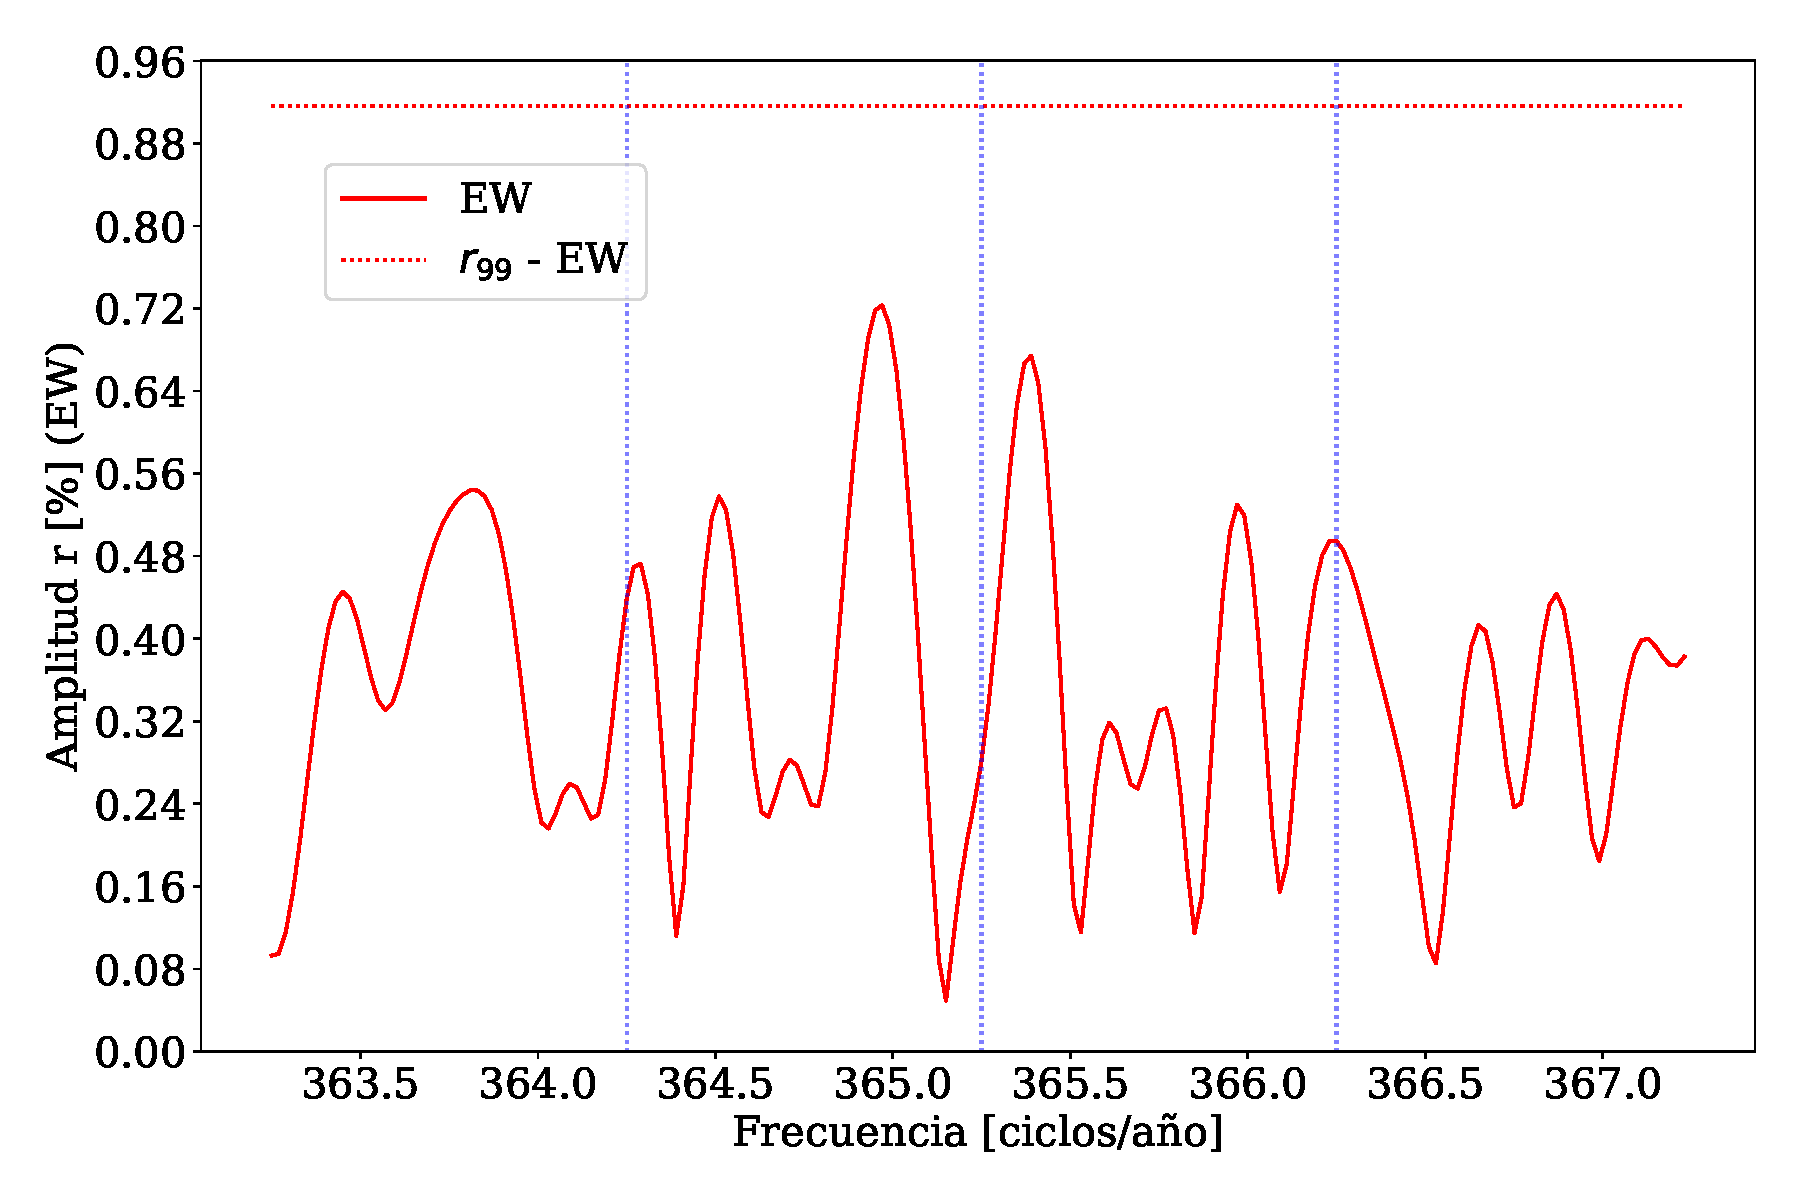
\includegraphics[width=0.75\textwidth]{plot_bin_3_barrido_v3_EW.pdf}
            \end{center}
            \caption{Barrido de frecuencias en el rango 1 EeV - 2 EeV .}
            \label{fig:tercer_barrido}
        \end{small}
    \end{figure}    

    \section{Gráficos}

    % Para poder comparar los resultados de $d_\perp$ entre sí, podríamos graficar los valores de la proyección y de la límite del $99\%$ como se muestra en la Fig.\ref{fig:no_normalizado}. El inconveniente es la cantidad de datos en cada rango de energía entre los conjuntos de datos, Todos los Disparos y Disparo Estándar, son distintos.


    % \begin{figure}[H]
    %     \begin{small}
    %         \begin{center}
    %             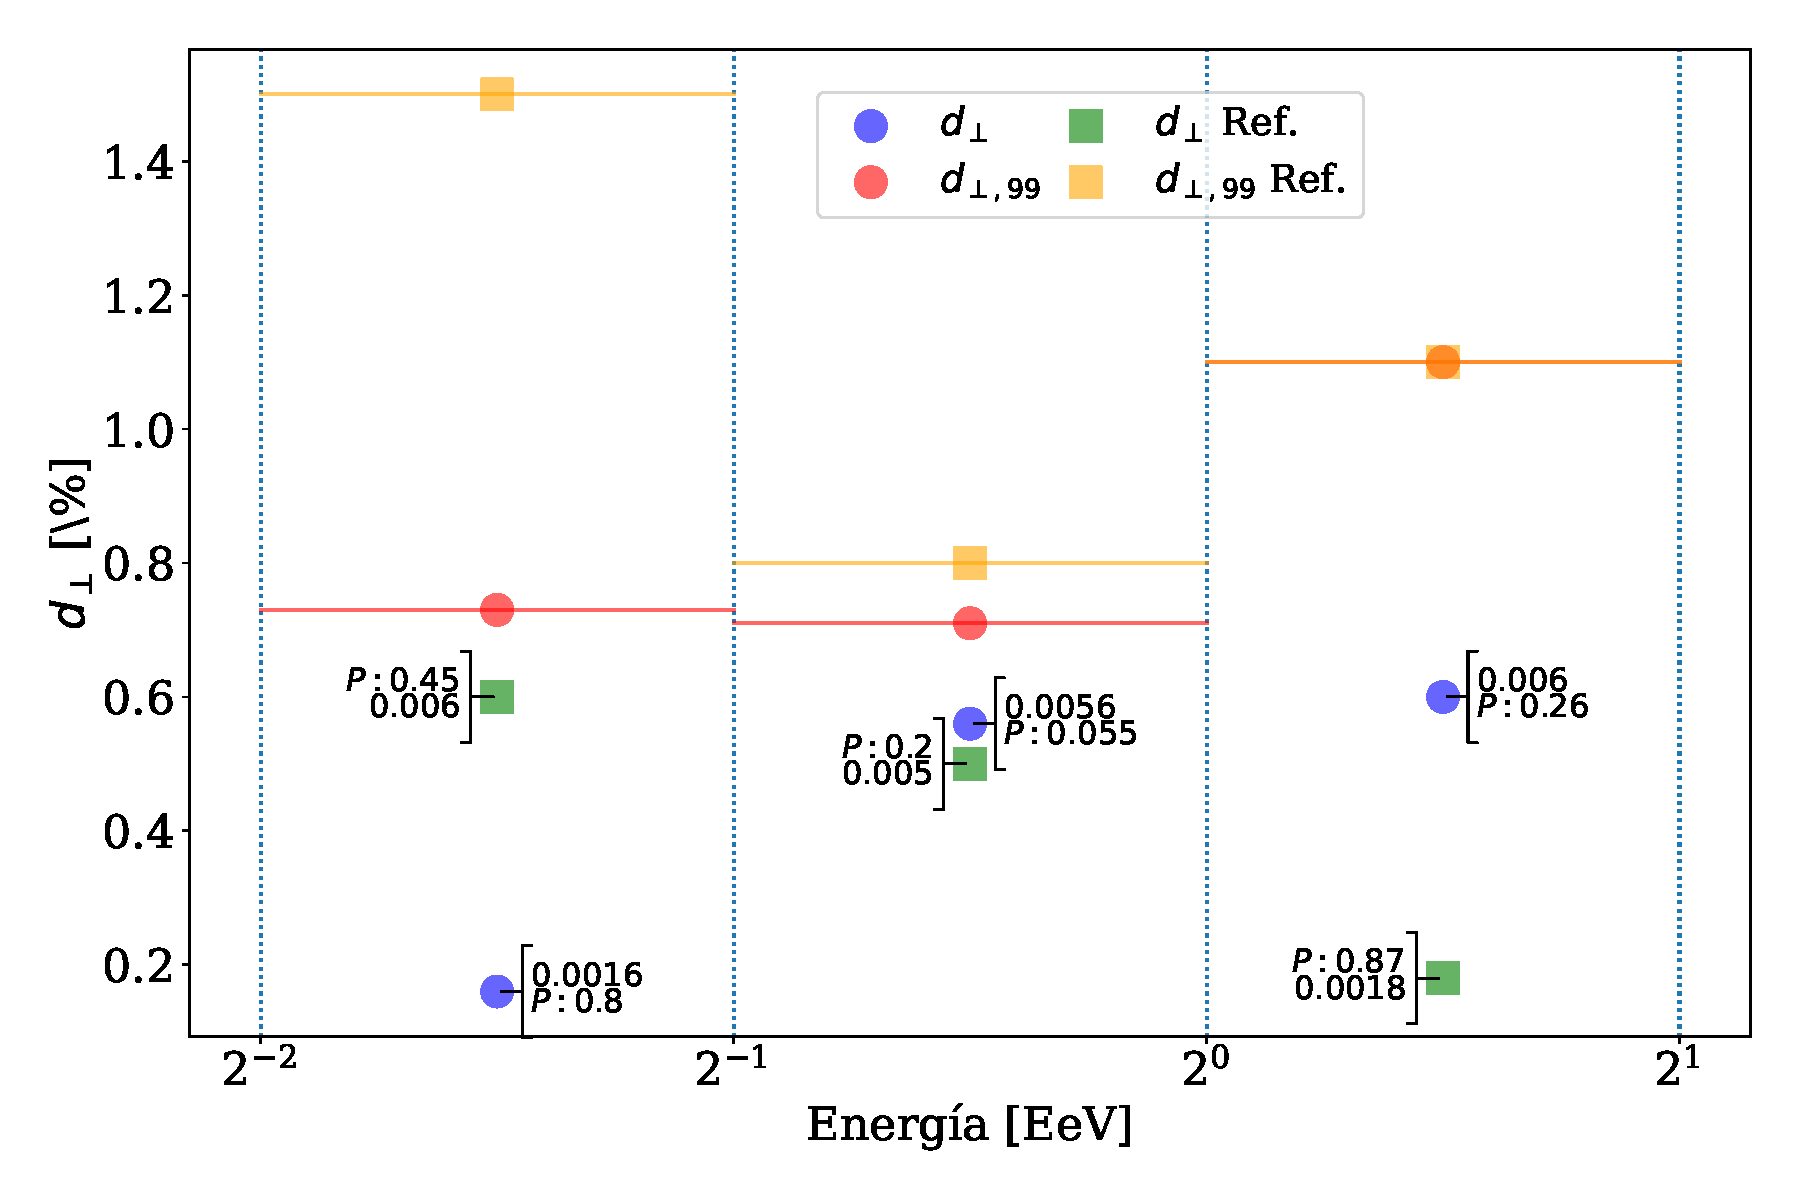
\includegraphics[width=0.75\textwidth]{d_perp_no_normalizado_v4.pdf}
    %         \end{center}
    %         \caption{Sin normalizar}
    %         \label{fig:no_normalizado}
    %     \end{small}
    % \end{figure}
    
    % Para compararlos mejor con respecto a $d_{\perp,UL}$, usamos el valor de cada rango y de cada conjunto de datos, para normalizar la amplitud de $d_{\perp,UL}$. Como se muestra en la Fig.\ref{fig:normalizado}, ahora $d_{\perp,UL}=1$ y los otros valores se pueden comparar. 

    % \begin{figure}[H]
    %     \begin{small}
    %         \begin{center}
    %             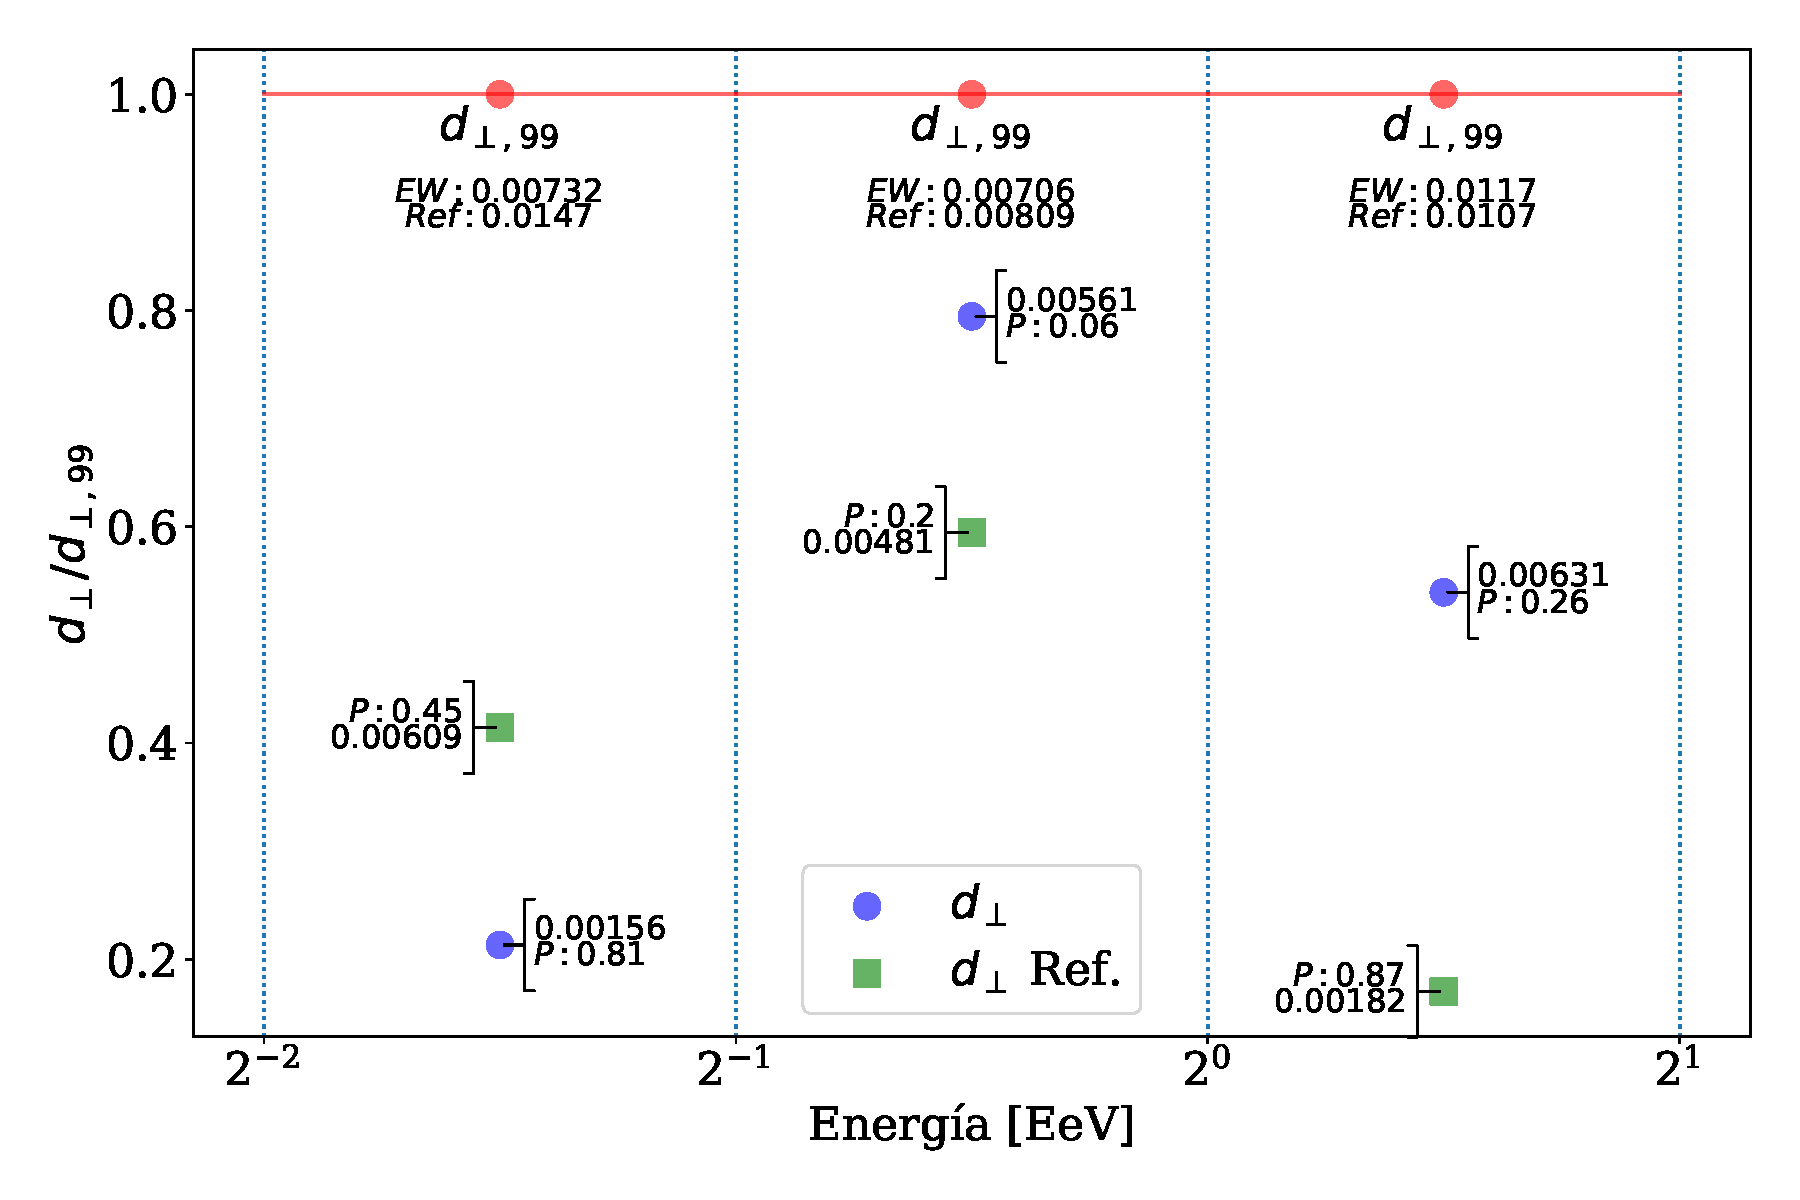
\includegraphics[width=0.75\textwidth]{d_perp_normalizado.pdf}
    %         \end{center}
    %         \caption{Valores normalizados con $d_{\perp,UL}$}
    %         \label{fig:normalizado}
    %     \end{small}
    % \end{figure}

    Una forma  para poder comparar los resultados de $d_\perp$ calculados de distintos conjuntos de  datos entre sí, es dividir estos valores con  sus respectivos $\sigma_{x,y}$. De esta manera, podemos comparar cuan apartados están con respecto $\sigma_{x,y}$, así se obtiene la Fig.\ref{fig:normalizado_sigma}.

    \begin{figure}[H]
        \begin{small}
            \begin{center}
                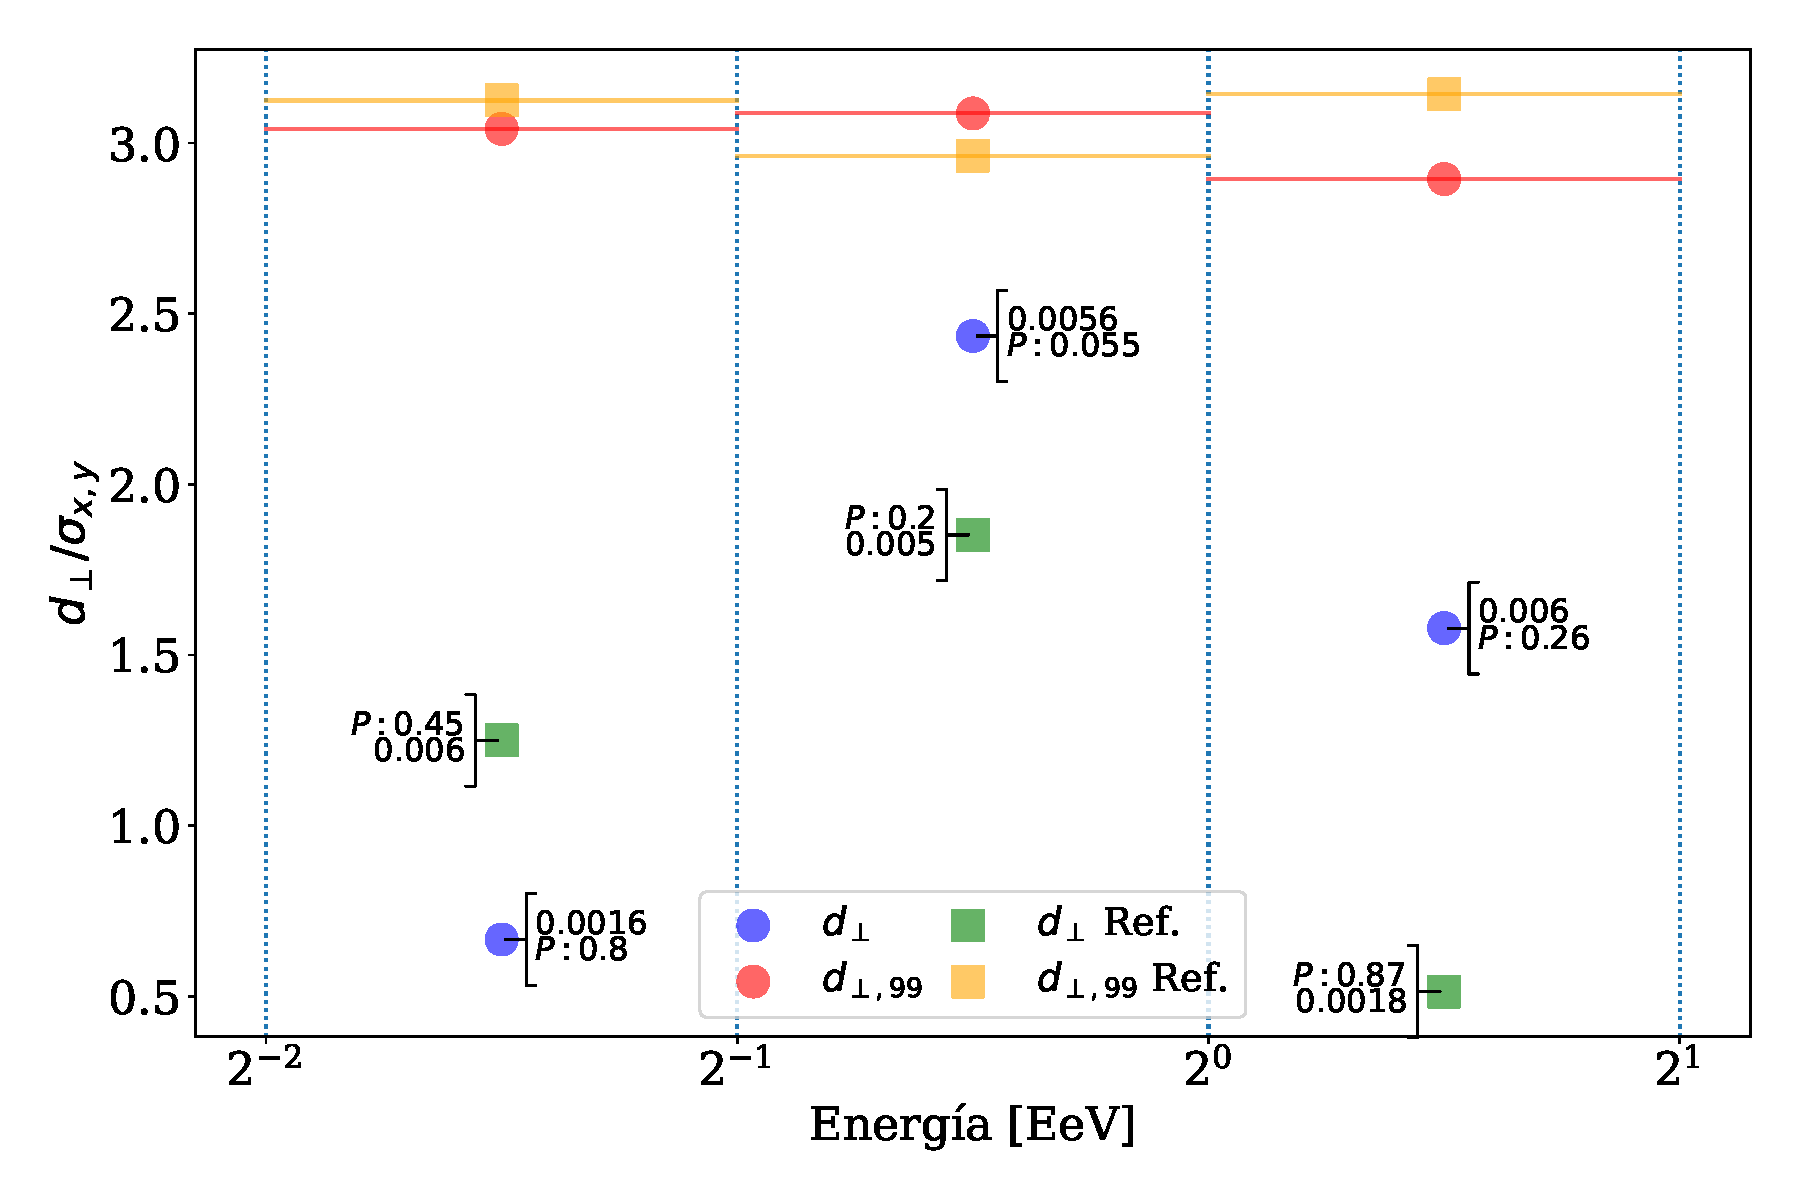
\includegraphics[width=0.75\textwidth]{d_perp_normalizado_sigmas_v5.pdf}
            \end{center}
            \caption{Valores normalizados con $d_{\perp,UL}$}
            \label{fig:normalizado_sigma}
        \end{small}
    \end{figure}

Por lo que ahora podemos decir que en los rangos entre 0.5 EeV - 1.0 EeV y 1.0 EeV - 2.0 EeV, la amplitud obtenida en este trabajo está por encima que en el trabajo \cite{Aab_2020} por $\sim 1\sigma_{x,y}$ y $\sim 2 \sigma_{x,y}$ respectivamente.

Para comparar los resultados en el  rango 0.25 EeV - 0.5 EeV, tenemos que tener en cuenta que el Disparo Estándar tiene una sensibilidad menor que el Todos los Disparos. Esto se ve claramente en la Tabla \ref{tab:datasets}, donde el primero tiene 7 veces menos eventos para analizar que el segundo. Por lo tanto, la discrepancia entre en el trabajo \cite{Aab_2020} y los trabajos puede deberse a la  diferencia de eventos a estudiar causada por la sensibilidad del disparo.


Considerando los valores de $\sigma_{x,y}$ y $d_\perp$ obtenidos para cada rango de energía, es posible  comparar las direcciones, valores e incertidumbres en la Fig.\ref{fig:incertidumbre}. Las líneas punteadas están centradas en los valores reportados en el trabajo \cite{Aab_2020} en cada rango de energía y con radio igual a sus $\sigma_{x,y}$ . 

\begin{figure}[H]
    \begin{small}
        \begin{center}
            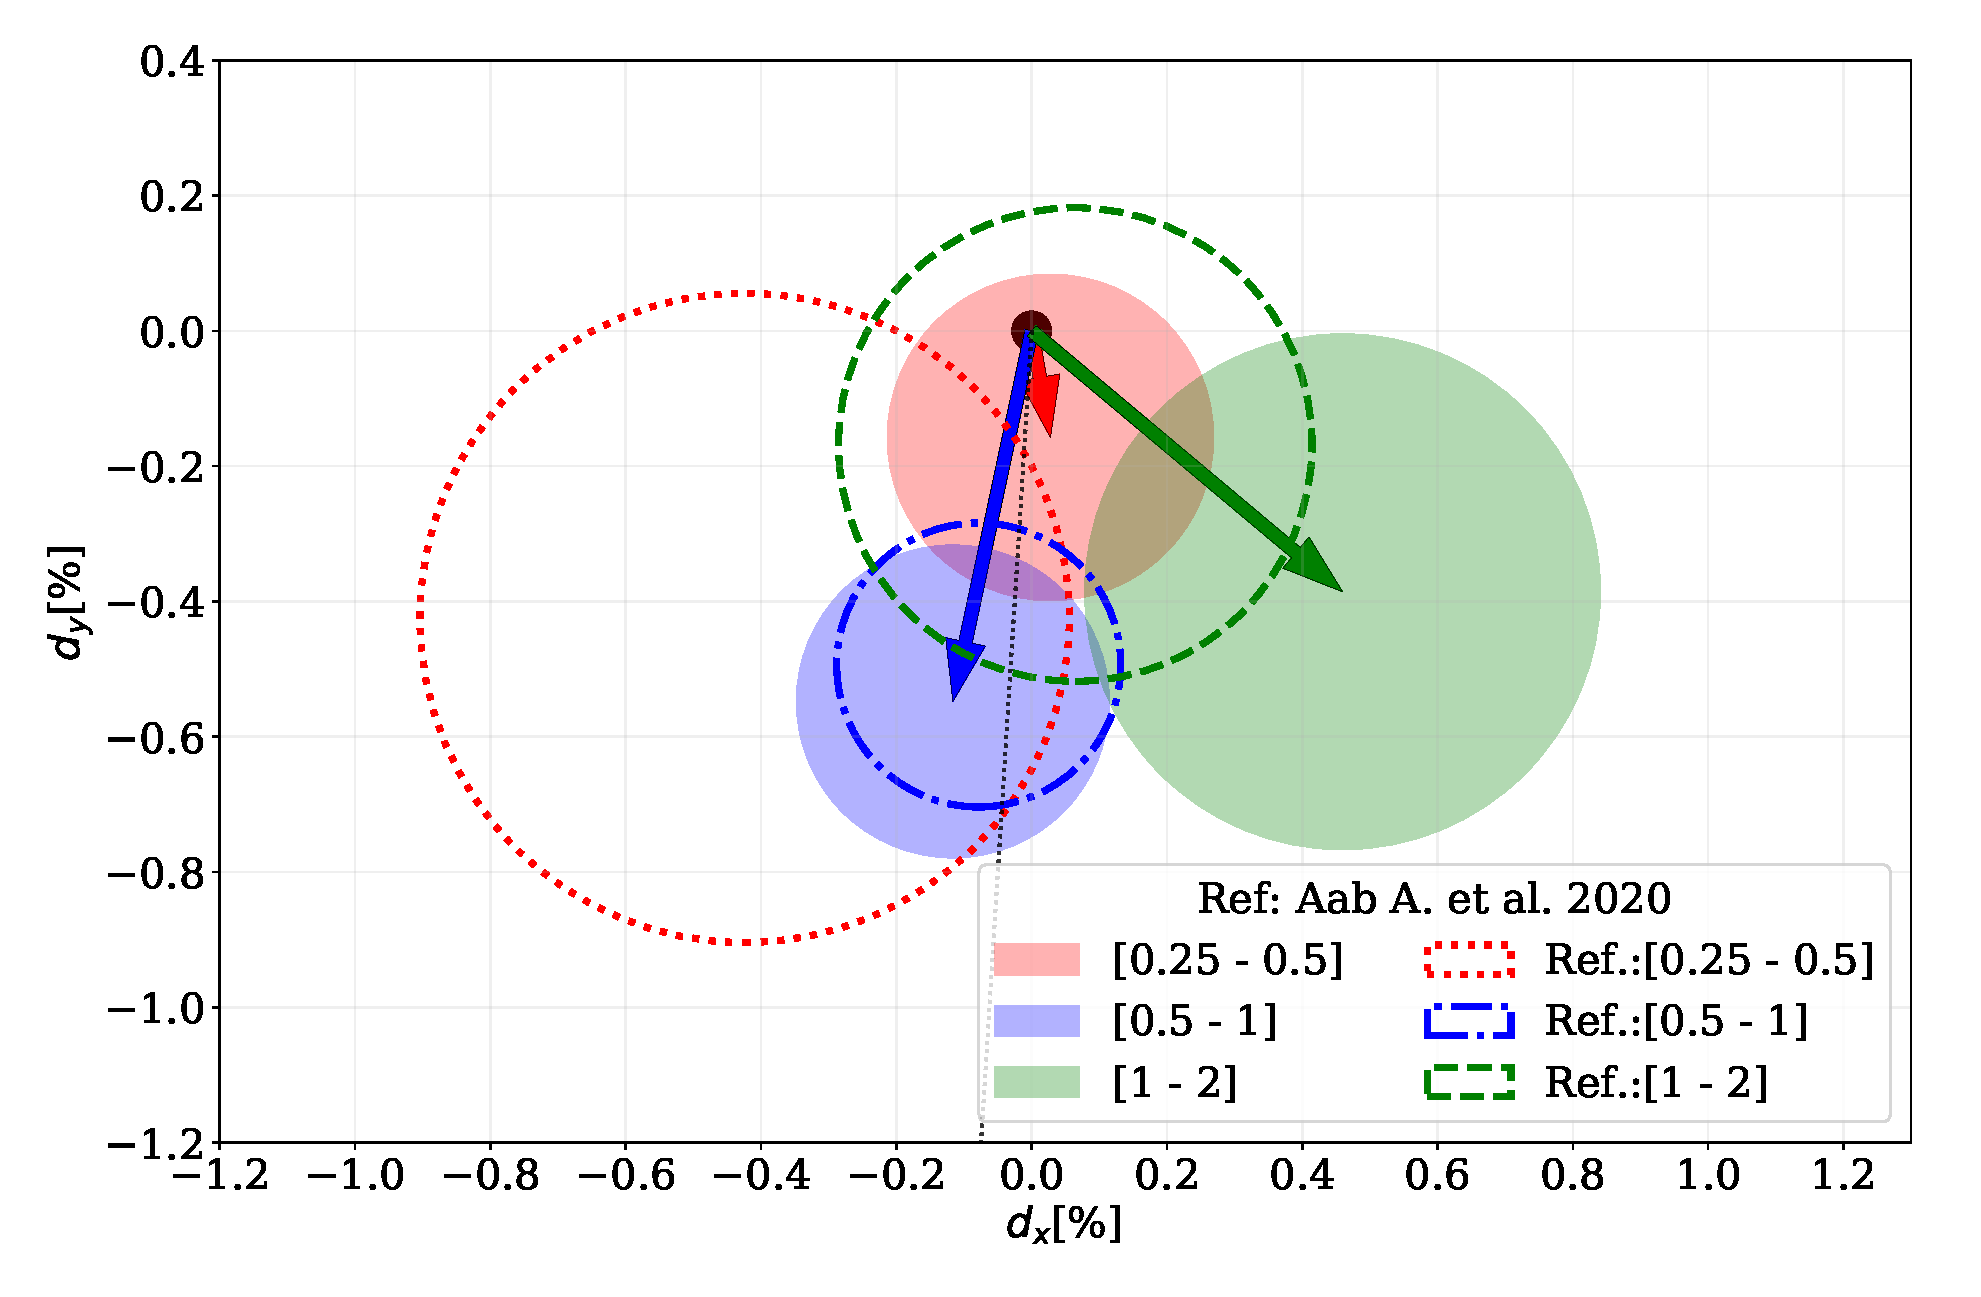
\includegraphics[width=0.9\textwidth]{comparando_sigmas_v3.pdf}
        \end{center}
        \caption{Amplitudes con incertidumbre, apuntando en la dirección  de la fase. Los círculos punteados los valores del trabajo \cite{Aab_2020}del trabajo \cite{Aab_2020} con sus respectivas incertidumbres y la línea punteada en negro marca la dirección del centro galáctico.}
        \label{fig:incertidumbre}
    \end{small}
\end{figure}


\chapter{Esto va a ir en otro capítulo que todavía no armé. Y los resultados no estan actualizados}
\section{Comparando resultados entre métodos para barridos de frecuencias}

\section{Verificación del código escrito durante la maestría}

Para ver que todo cierre, obtuve los resultados del paper \cite{Aab_2020} con el código del Rayleigh para distintos bines. En el bin  2 EeV - 4 EeV  tuve incongruencias entre mi código y los valores reportados en el paper, pero si comparo los valores obtenidos con el código utilizado para el paper con mis resultados si se corresponden. En los demás bines los resultados entre el código implementado en \cite{Aab_2020}, los resultados publicados y los resultados de mi código se corresponden.


En el bin 2 EeV - 4 EeV, verifiqué sin cambiaba los números considerando los eventos hasta $80^o$, pero los parámetros de Rayleigh eran los mismos que usar $60^o$  como límite en $\theta$.  Cuando no considero los pesos en mi código, obtengo resultados congruentes con los publicados pero eso puedo ser una casualidad.

\begin{table}[H]
    \begin{small}
        \begin{center}
            \begin{tabular}[c]{l|c|c|c|c|}
                                            & \multicolumn{4}{|c|}{2 EeV - 4 EeV}                                                               \\ \hline
                Frecuencia:                 & Sidérea              & Sidérea (Sin pesos)  & Sidérea \cite{codigo}    & Sidérea \cite{Aab_2020}   \\ \hline
                Amplitud r [\%]:            & $0.5^{+0.3}_{-0.2}$ & $0.4^{+0.3}_{-0.2}$ & $0.5^{+0.3}_{-0.2}$     & -                          \\
                $r_{99}$ [\%]:              & 0.8                 & 0.8                 & 0.8                     & -                          \\\hline
                Amplitud $d_\perp$[\%]:     & $0.7^{+0.4}_{-0.2}$ & $0.5^{+0.4}_{-0.2}$ & $0.7^{+0.4}_{-0.2}$ 	  & $0.5^{+0.4}_{-0.2}$                    \\
                $d_{99}$ [\%]:              & 1.0                 & 1.0                 & 1.0                     & -                         \\
                $d_{\perp,UL}$[\%]:         & 1.9                 & 1.7                 & -                       & 1.4                               \\\hline
                $\sigma_{x,y}$[\%]:         & 0.34	              & 0.34	            & 0.34	                  & 0.34                           \\
                Probabilidad      :         & 0.14                & 0.33                & 0.15               	  & 0.34                       \\
                Fase[$^o$]:                 & 355$\pm$29          & 351$\pm$38          & 346$\pm$29              & 349$\pm$55                    \\\hline
            \end{tabular}
        \end{center}
    \end{small}
    \caption{Características para las frecuencias solar y sidérea con el método Rayleigh en el primer armónico en el rango de energía 2 EeV - 4 EeV, obtenidos con el código de este trabajo \cite{Aab_2020} y comparados con los resultados reportados en el último.}
\end{table}


\begin{table}[H]
    \begin{small}
        \begin{center}
            \begin{tabular}[c]{l|c|c||c|c|}
                                            & \multicolumn{2}{c||}{8 EeV - 16 EeV}              & \multicolumn{2}{c|}{16 EeV - 32 EeV}                   \\ \hline
                Frecuencia:                 & Sidérea                    & Sidérea \cite{Aab_2020} & Sidérea                   & Sidérea \cite{Aab_2020}   \\ \hline
                Amplitud r [\%]:            & $4.4^{+1.0}_{-0.8}$ 	    & -                      & $5.8^{+1.8}_{-1.3}$ 	    & -                         \\
                $r_{99}$ [\%]:              & 2.6                       & -                      & 4.9                      & -                          \\\hline
                Amplitud $d_\perp$[\%]:     & $5.6^{+1.2}_{-1.0}$ 	    & $5.6^{+1.2}_{-1.0}$    & $7.5^{+2.3}_{-1.8}$ 	    & $7.5^{+2.3}_{-1.8}$                   \\
                $d_{99}$ [\%]:              & 3.3                       & -                      & 6.3                      & -                         \\
                $d_{\perp,UL}$[\%]:         & 10                        & -                      & 16                       & -                                 \\\hline
                $\sigma_{x,y}$[\%]:         & 1.1	                    & 1.1                    & 2.1	                    & 2.1                           \\
                Probabilidad      :         & $2.3\times10^{-6}$	    & $2.3\times10^{-6}$     & $1.5\times10^{-3}$	    & $1.5\times10^{-3}$              \\
                Fase[$^o$]:                 & 96$\pm$11                 & 97$\pm$12              & 80$\pm$16                & 80$\pm$17                     \\\hline
            \end{tabular}
        \end{center}
    \end{small}
    \caption{Características para las frecuencias solar y sidérea con el método Rayleigh en el primer armónico en distintos rangos de energía, obtenidos con el código de este trabajo \cite{Aab_2020} y comparados con los resultados reportados en el último.}
\end{table}


\section{Comparando amplitud en función de la frecuencia}

En las Figs.\ref{fig:primer_barrido_EW_Ray}, \ref{fig:segundo_barrido_EW_Ray} y \ref{fig:tercer_barrido_EW_Ray} se comparan el barrido en frecuencia con el método East - West y el barrido con Rayleigh considerando los pesos de los hexágonos en distintos rangos de energía.


\begin{figure}[H]
    \begin{small}
        \begin{center}
            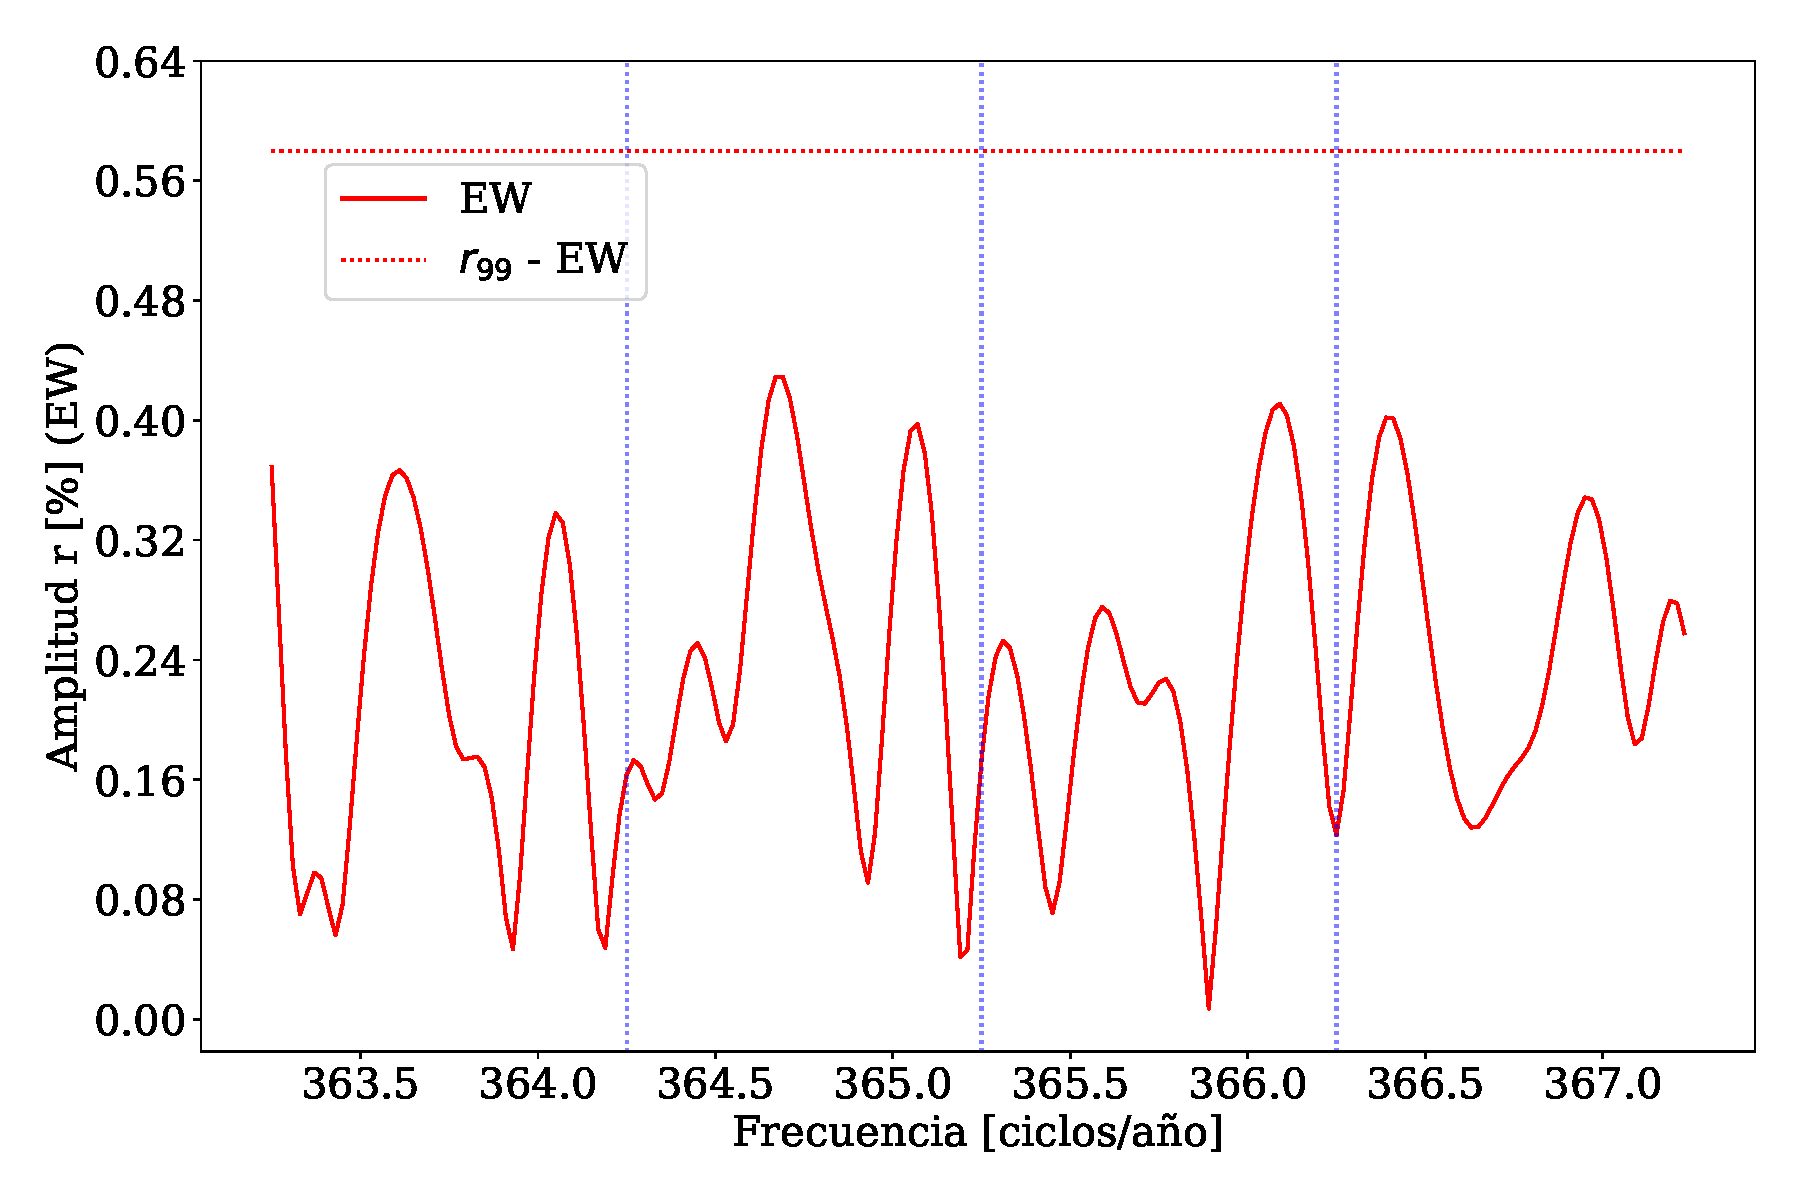
\includegraphics[width=0.4955\textwidth]{plot_bin_1_barrido_v3_EW.pdf}
            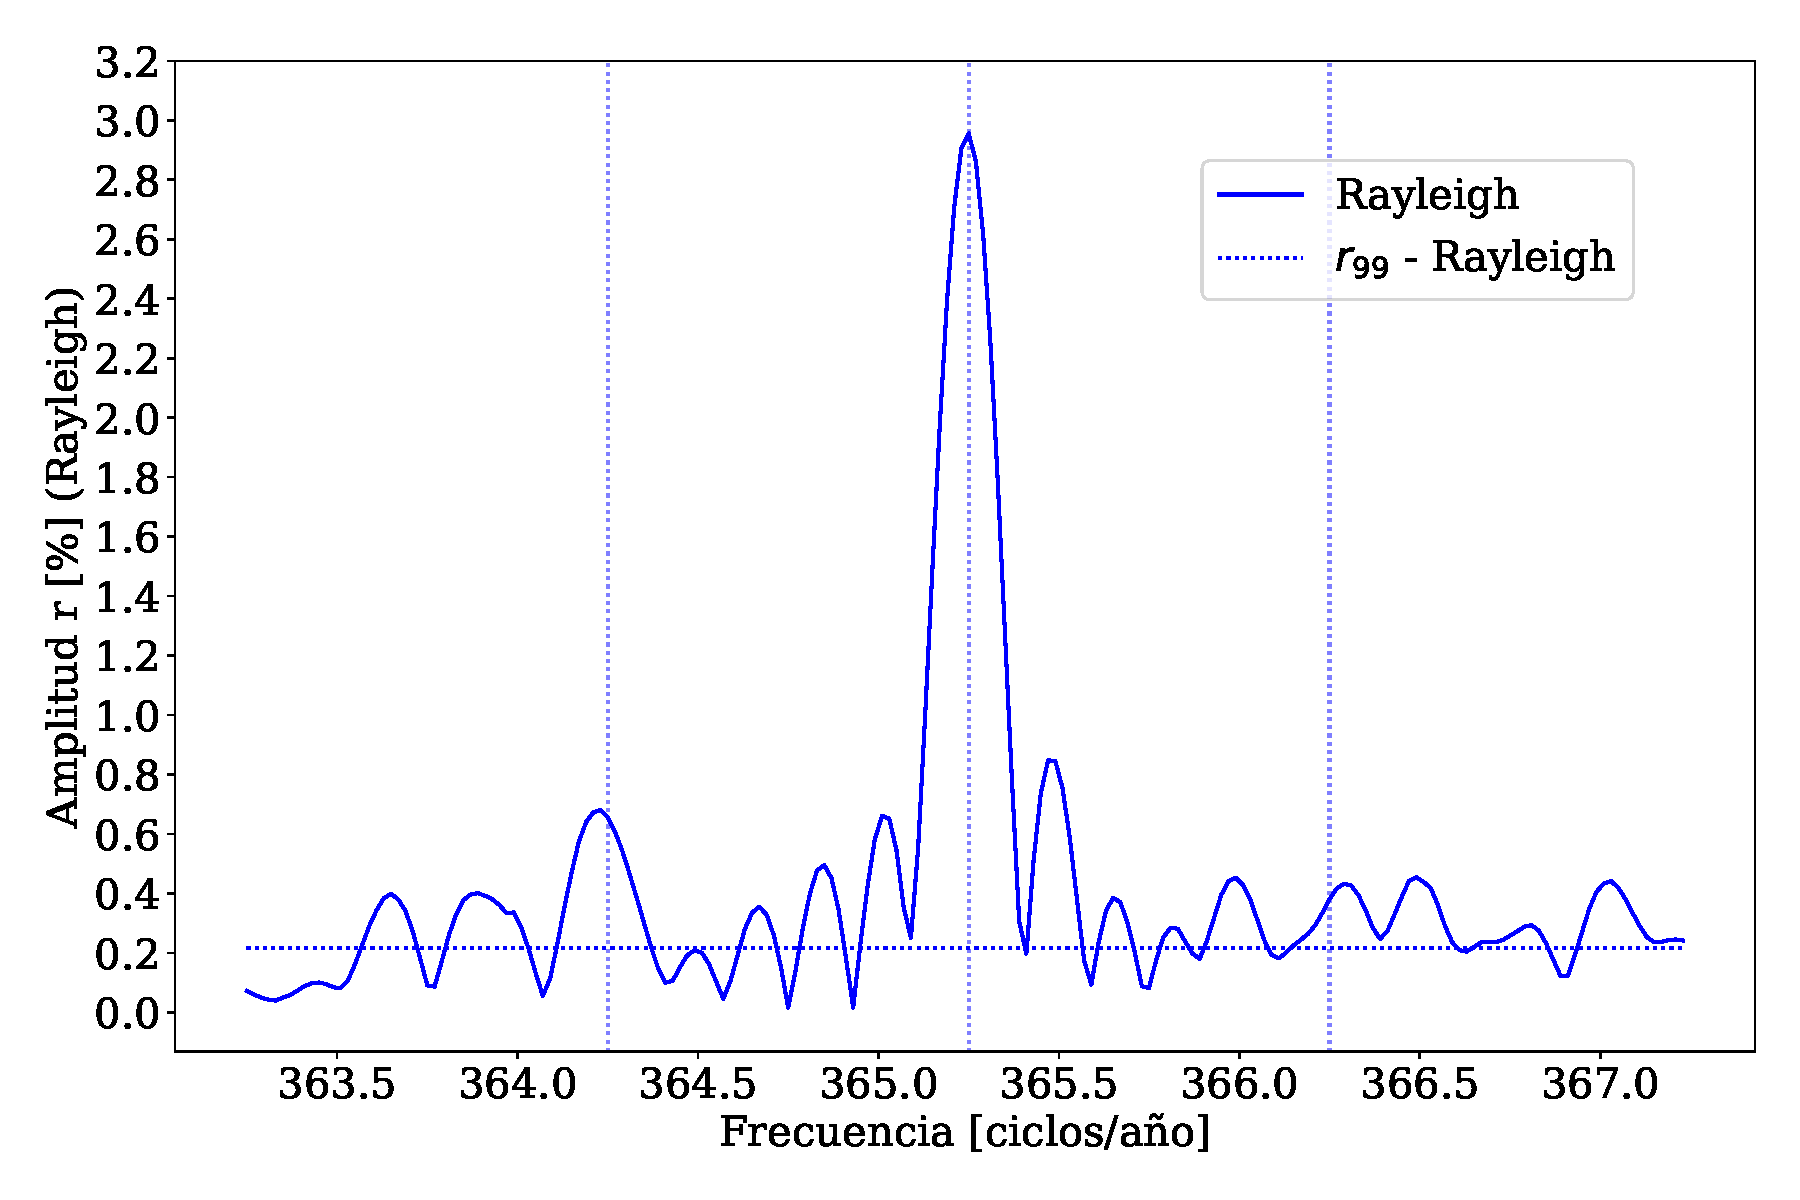
\includegraphics[width=0.4955\textwidth]{plot_bin_1_barrido_v1_Ray.pdf}
        \end{center}
        \caption{Barrido de frecuencias en el rango 0.25 EeV - 0.5 EeV .}
        \label{fig:primer_barrido_EW_Ray}
    \end{small}
\end{figure}    

\begin{figure}[H]
    \begin{small}
        \begin{center}
            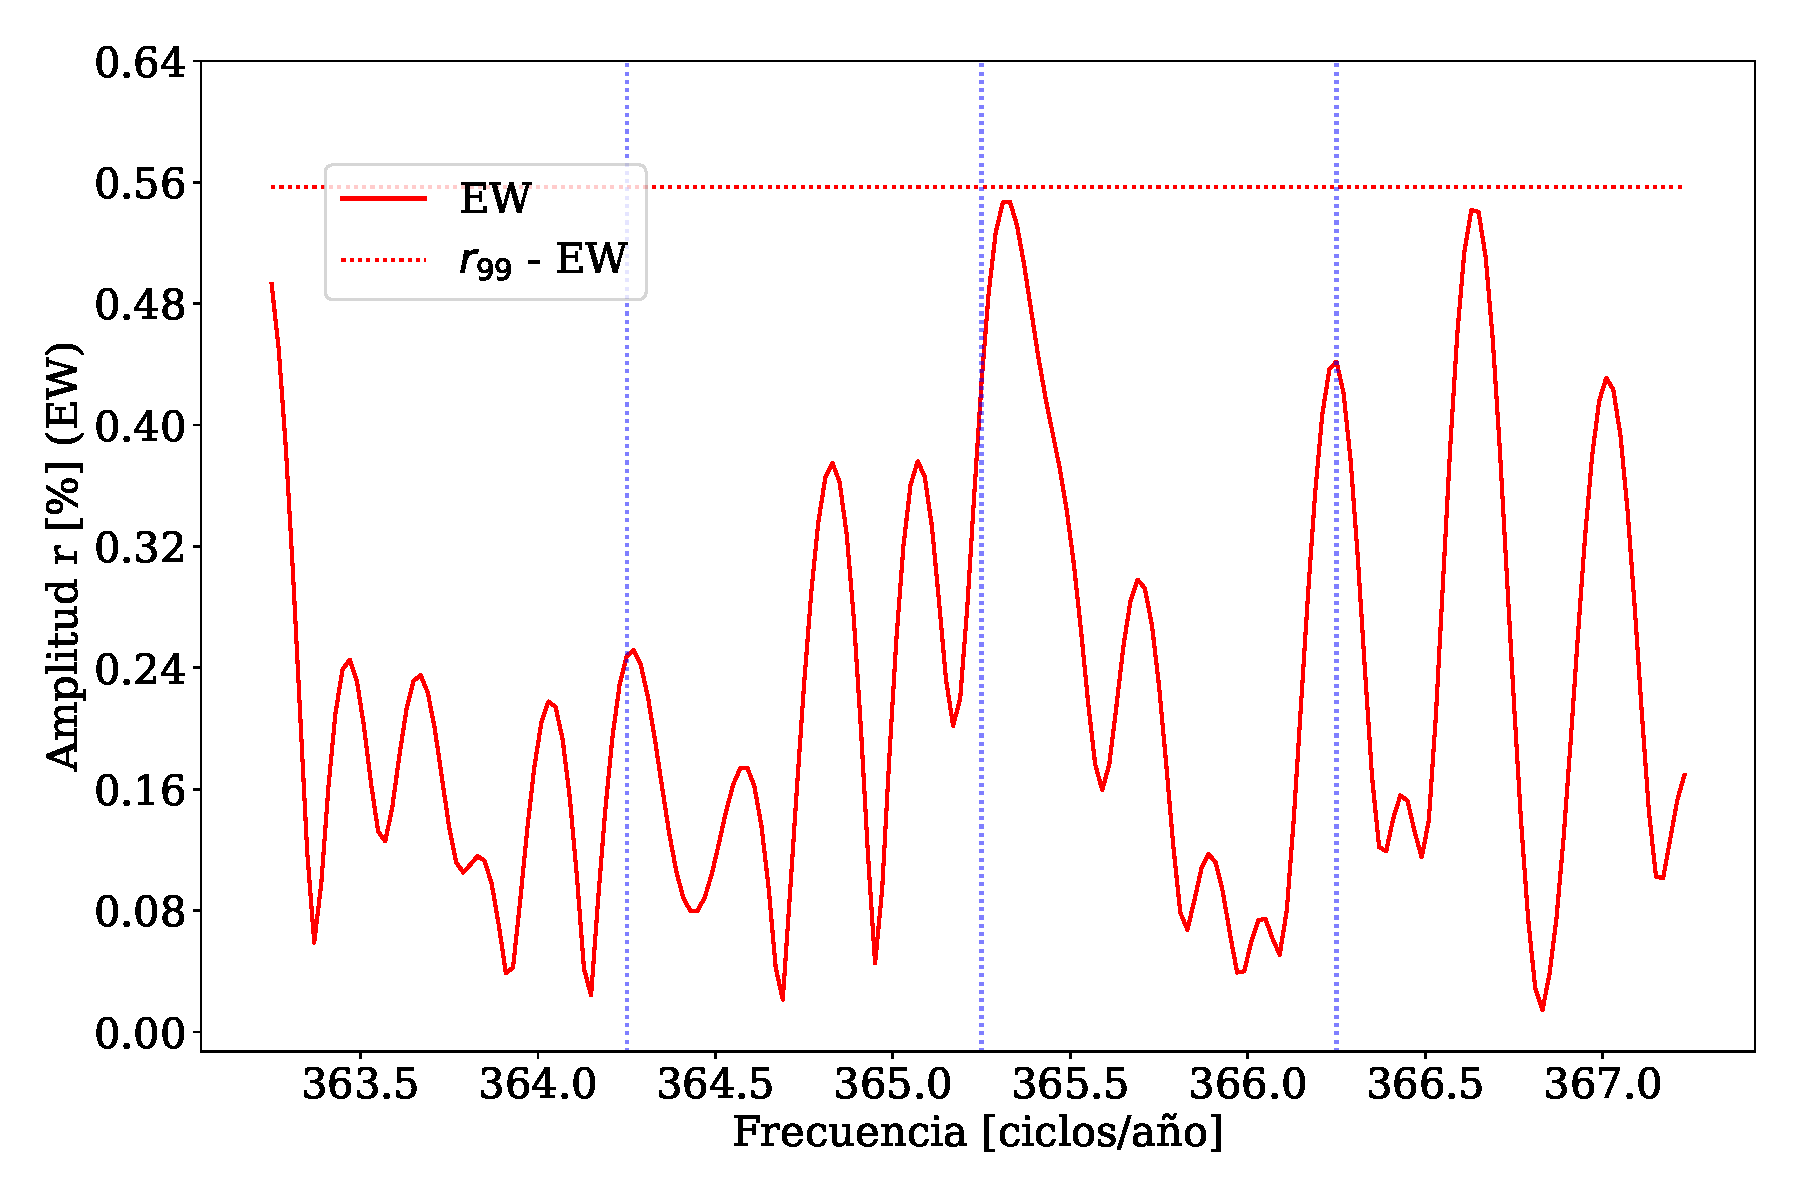
\includegraphics[width=0.4955\textwidth]{plot_bin_2_barrido_v3_EW.pdf}
            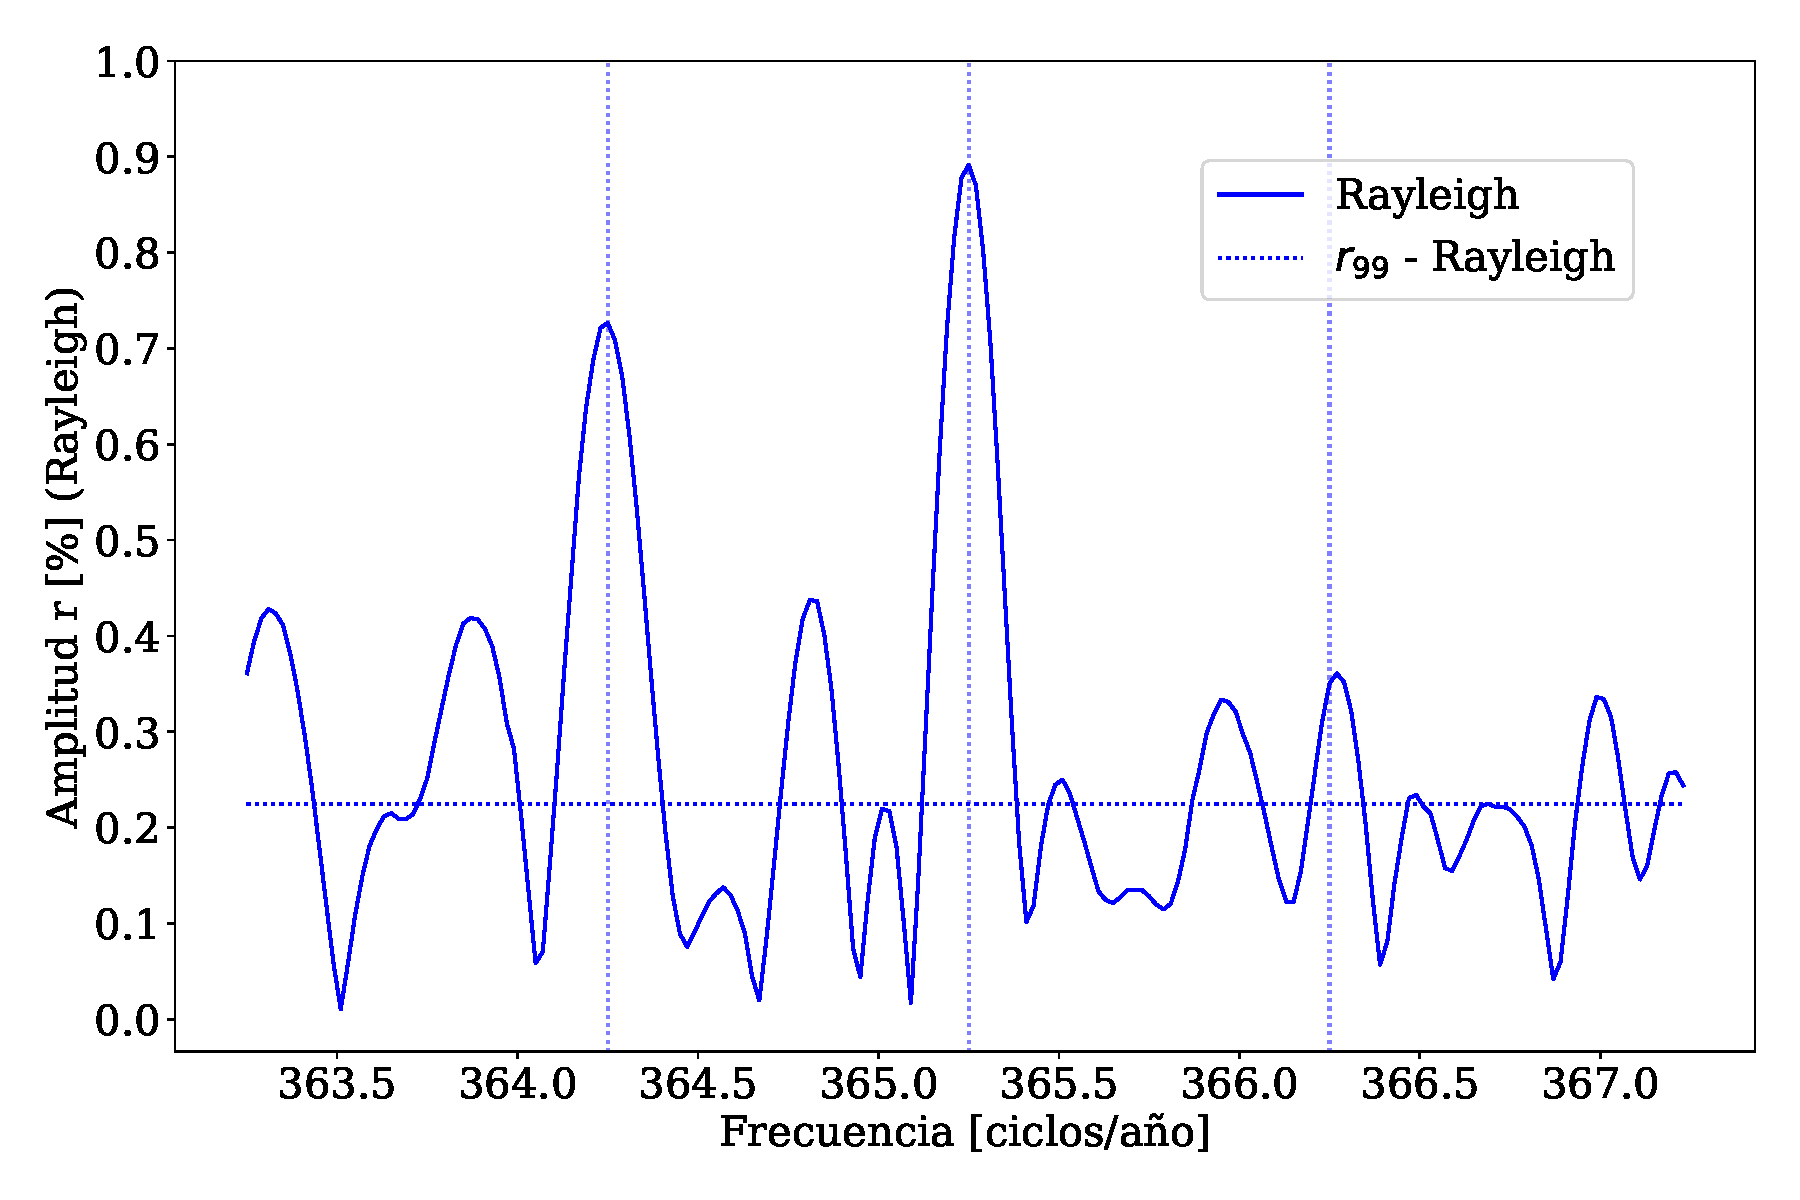
\includegraphics[width=0.4955\textwidth]{plot_bin_2_barrido_v1_Ray.pdf}
        \end{center}
        \caption{Barrido de frecuencias en el rango 0.5 EeV - 1 EeV .}
        \label{fig:segundo_barrido_EW_Ray}
    \end{small}
\end{figure}    

\begin{figure}[H]
    \begin{small}
        \begin{center}
            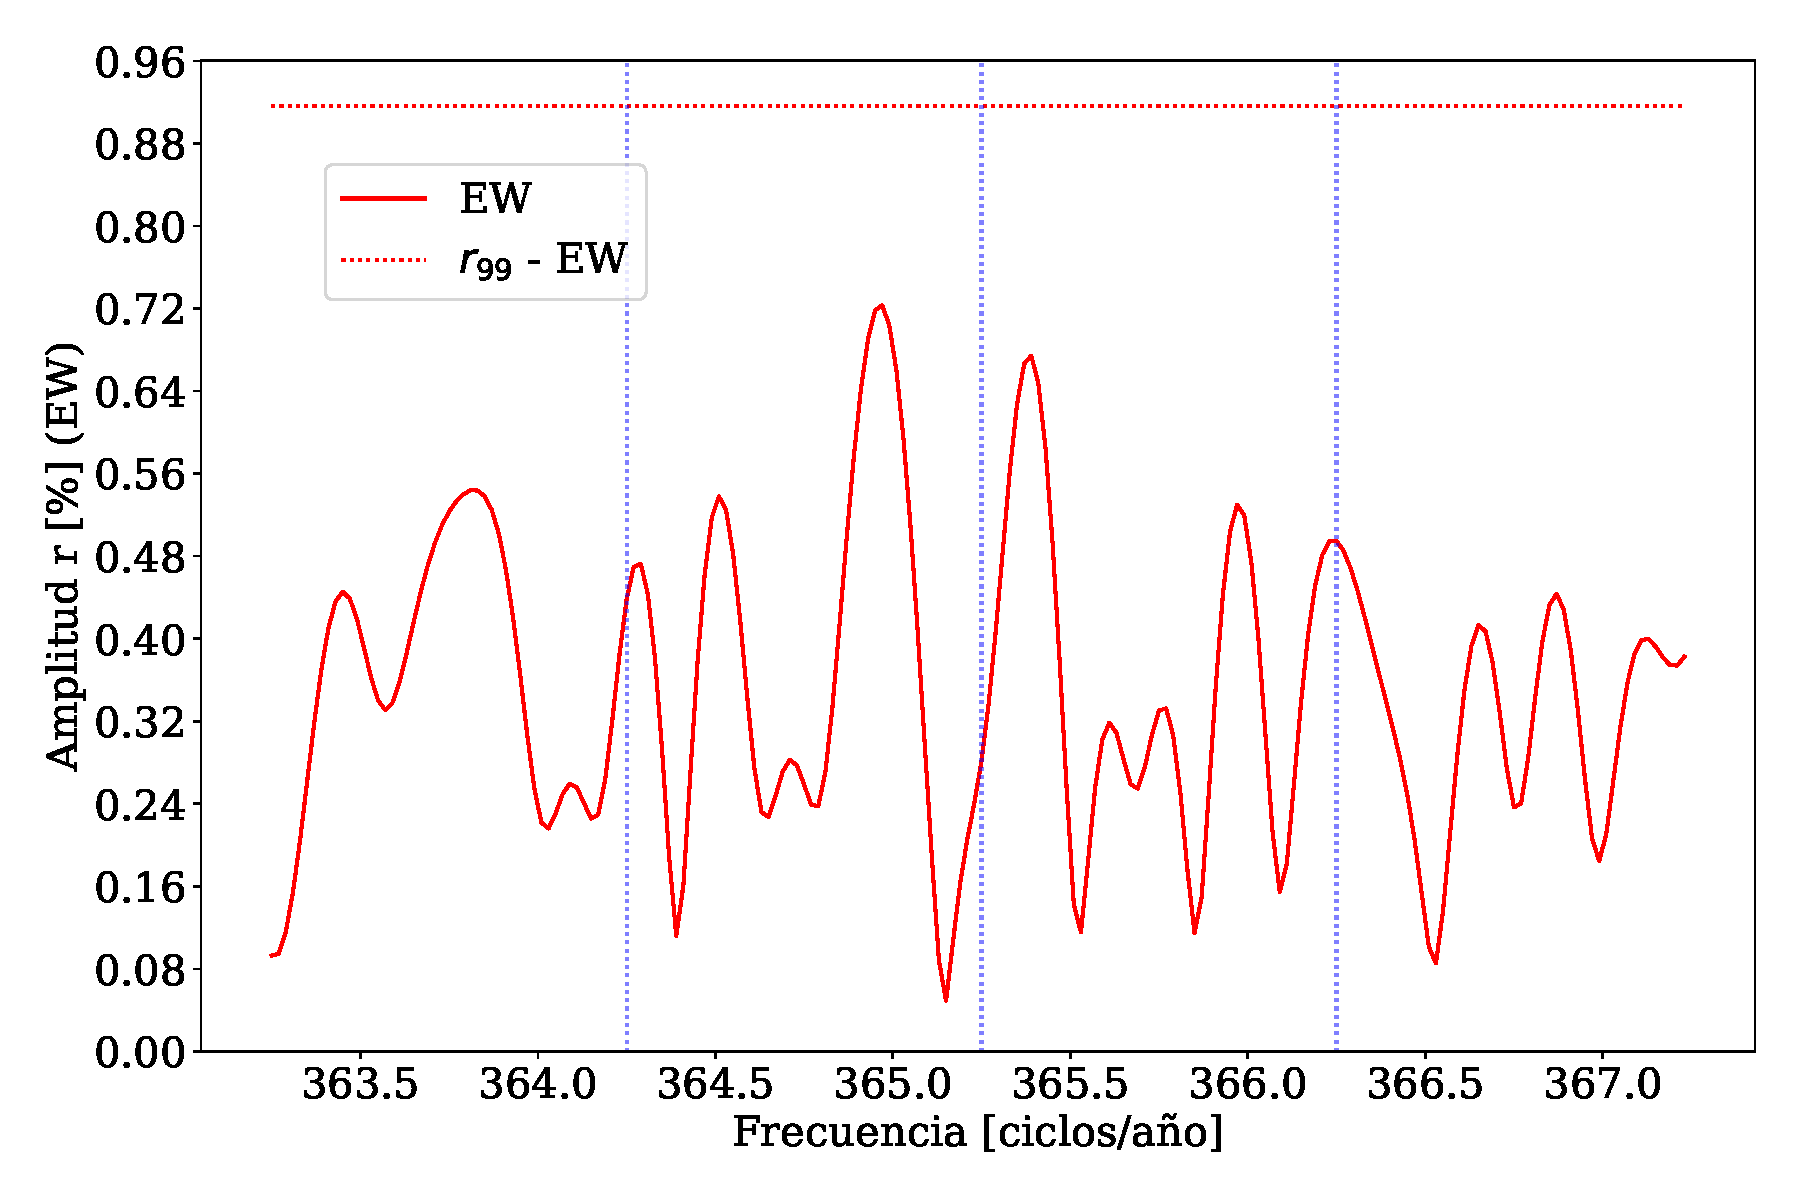
\includegraphics[width=0.4955\textwidth]{plot_bin_3_barrido_v3_EW.pdf}
            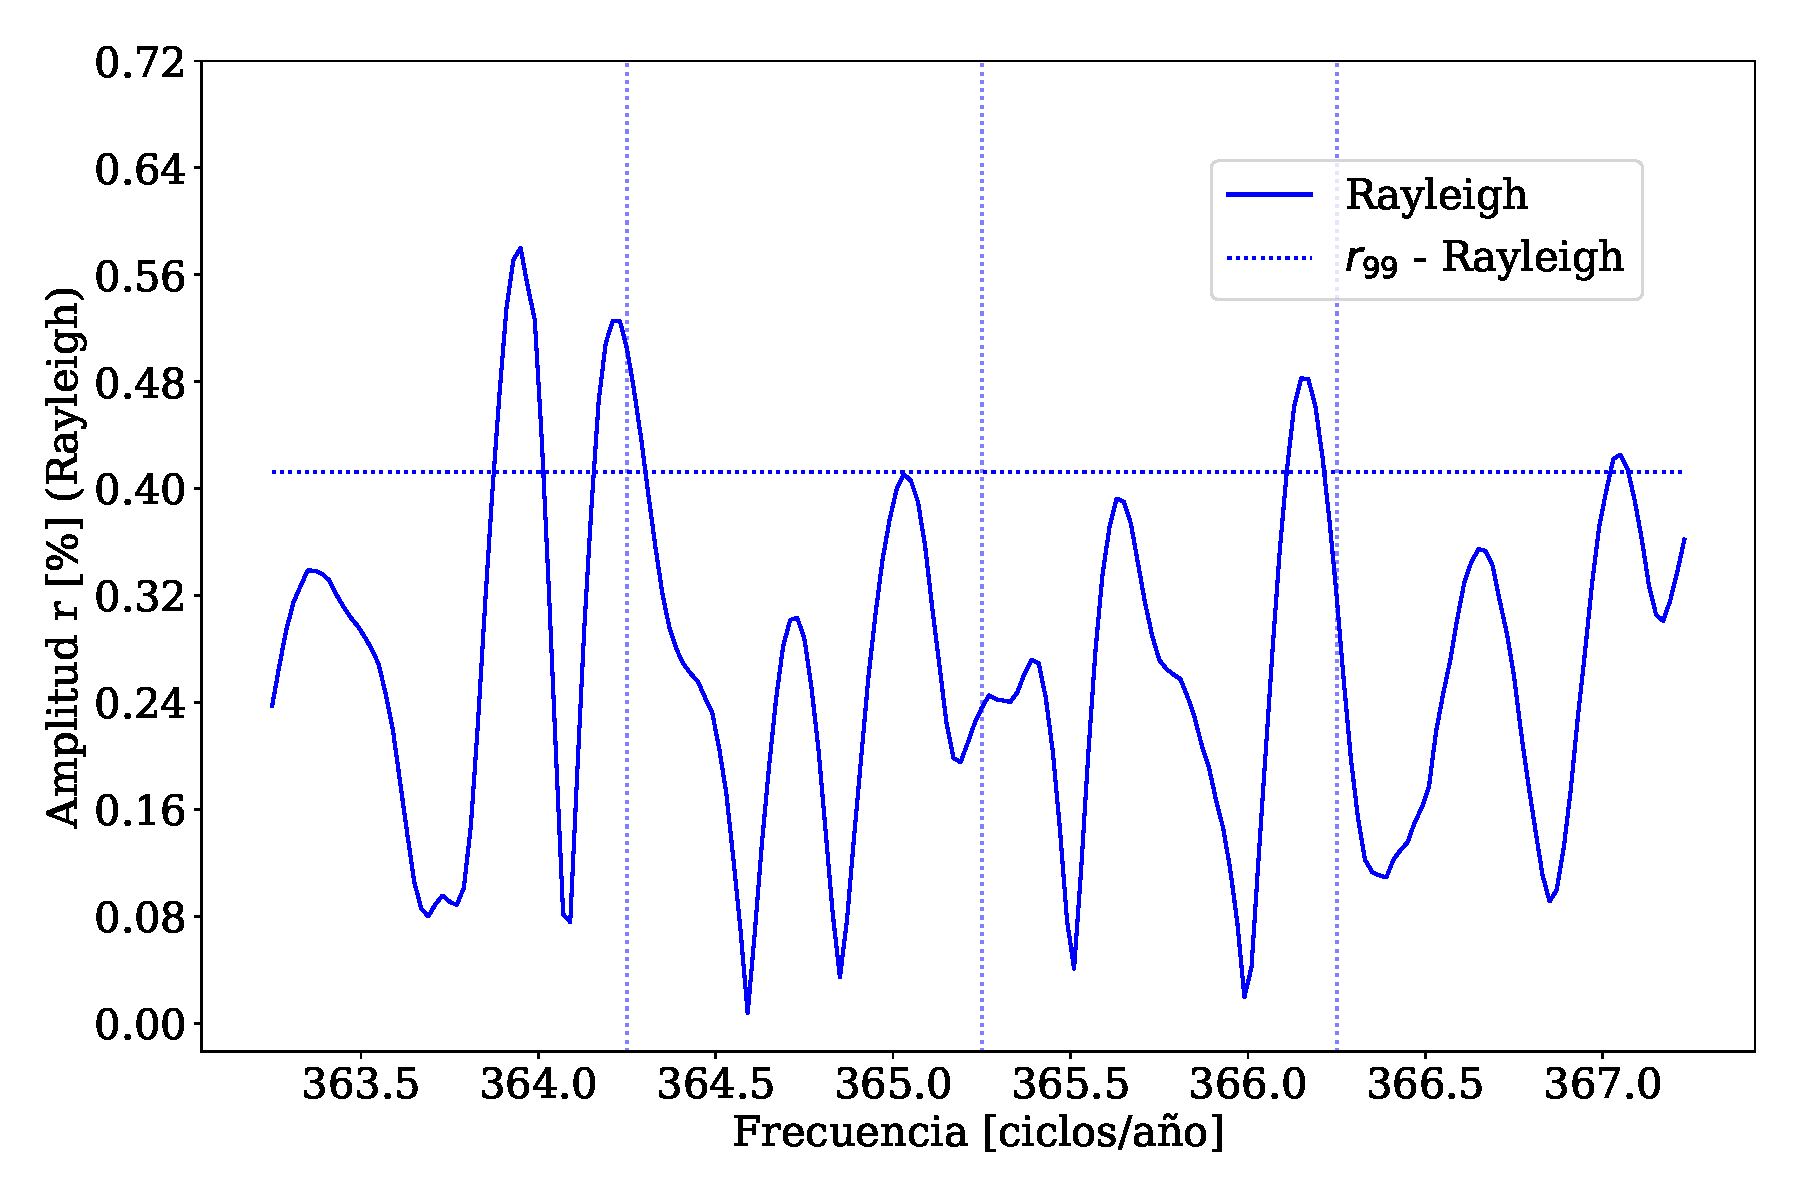
\includegraphics[width=0.4955\textwidth]{plot_bin_3_barrido_v1_Ray.pdf}
        \end{center}
        \caption{Barrido de frecuencias en el rango 1 EeV - 2 EeV .}
        \label{fig:tercer_barrido_EW_Ray}
    \end{small}
\end{figure}    

